%导演区
\documentclass[a4paper,11pt,UTF8]{article}%book,report,letter
\usepackage[table]{xcolor}
\usepackage{ctex}
\usepackage{geometry}
\geometry{a4paper,scale=0.8}
\usepackage{amsfonts}
\usepackage{amssymb}
\usepackage{verbatim}
\usepackage{mathrsfs}
\usepackage[arrow,matrix]{xy}
\usepackage{amsmath,amssymb,amscd,bm,bbm,amsthm,mathrsfs}
\usepackage{amsmath,amscd}
\usepackage{amsfonts,amssymb}
\usepackage{xypic}
\usepackage{indentfirst}
\usepackage{diagbox}
\usepackage{graphicx}
\usepackage{subfig}    %% 子图包
\usepackage{float} 
\usepackage{caption}
\captionsetup{labelfont=bf}
\usepackage{zhnumber} % change section number to chinese
%这下面为在latex中插入代码所需环境
\usepackage{CJK}
\usepackage{listings}
\usepackage{xcolor}
\lstset{
	language=Matlab,  %代码语言使用的是matlab
	frame=shadowbox, %把代码用带有阴影的框圈起来
	rulesepcolor=\color{red!20!green!20!blue!20},%代码块边框为淡青色
	keywordstyle=\color{blue!90}\bfseries, %代码关键字的颜色为蓝色,粗体
	commentstyle=\color{red!10!green!70}\textit,    % 设置代码注释的颜色
	showstringspaces=false,%不显示代码字符串中间的空格标记
	numbers=left, % 显示行号
	numberstyle=\tiny,    % 行号字体
	stringstyle=\ttfamily, % 代码字符串的特殊格式
	breaklines=true, %对过长的代码自动换行
	extendedchars=false,  %解决代码跨页时,章节标题,页眉等汉字不显示的问题
	texcl=true}
\def\d{\textup{d}}

\theoremstyle{plain}
\newtheorem{thm}{定理}[section]
\newtheorem{lem}{引理}[section]
\newtheorem{prop}{命题}[section]
\newtheorem{cor}{推论}[section]


\renewcommand{\qedsymbol}{$\square$}
\renewcommand\baselinestretch{1.25}
\renewcommand\thesection{\zhnum{section}}
\renewcommand \thesubsection {\arabic{section}}
%正文区
\begin{document}
	\title{\heiti 课题组组会-练习3}
	\author{王程 }
	\date{\today}
	\maketitle
	
	\section{练习及结果}
	1.对带源项的扩散方程$u_t=u_{xx}+\pi^2sin\left(\pi x\right),x\in \left[0,1\right],t\geq0$,满足以下初始条件$u\left(x,0\right)=x^2-x$,及边界条件$u\left(0,t\right)=u\left(1,t\right)=0$.\\
	\indent(1)将空间离散格式改为DG(P0P1)+DG(P0),时间离散方式使用a)显式欧拉格式,b)TVD-RK3,c)BDF1在均匀网格下进行求解。\\
	\indent(2)在网格生成时,对内部点坐标进行随机扰动,扰动范围为$\pm5\%\Delta x_{uniform}$,重新对问题进行求解,并测试精度。\\
	\indent 2在$x\in \left[0,1\right]$的均匀网格上尝试使用Green-Gauss Reconstruction 对$f\left(x\right)$及$g\left(x\right)$进行P1P2重构,其中$f\left(x\right)=1+x+x^2$,$g\left(x\right)=sin\left(\pi x\right)$,测试重构精度。如果网格为不均匀网格呢? \\
	~\\
	
	\textbf{解:}\\
	\indent(1)更改空间离散格式,下面给出三种时间离散格式下(单元格数为8,64)的方程数值解与解析解对比图以及空间精度。\\
	A)\textbf{Explicit Euler}\\
		\begin{figure}[!h]
		\centering
		\subfloat[8 elements]{
			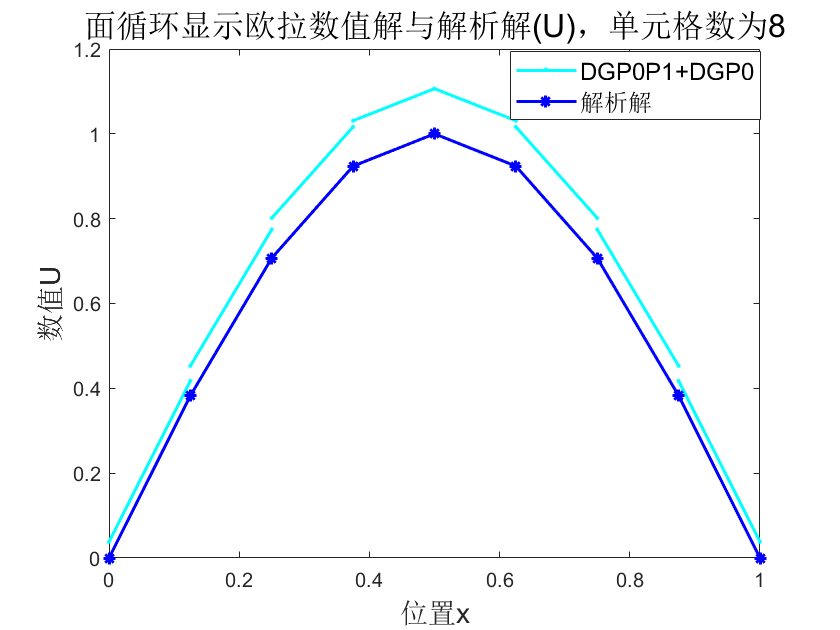
\includegraphics[width=3in]{obviouseuler/U8.png} 
		}
		\hfill
\subfloat[64 elements]{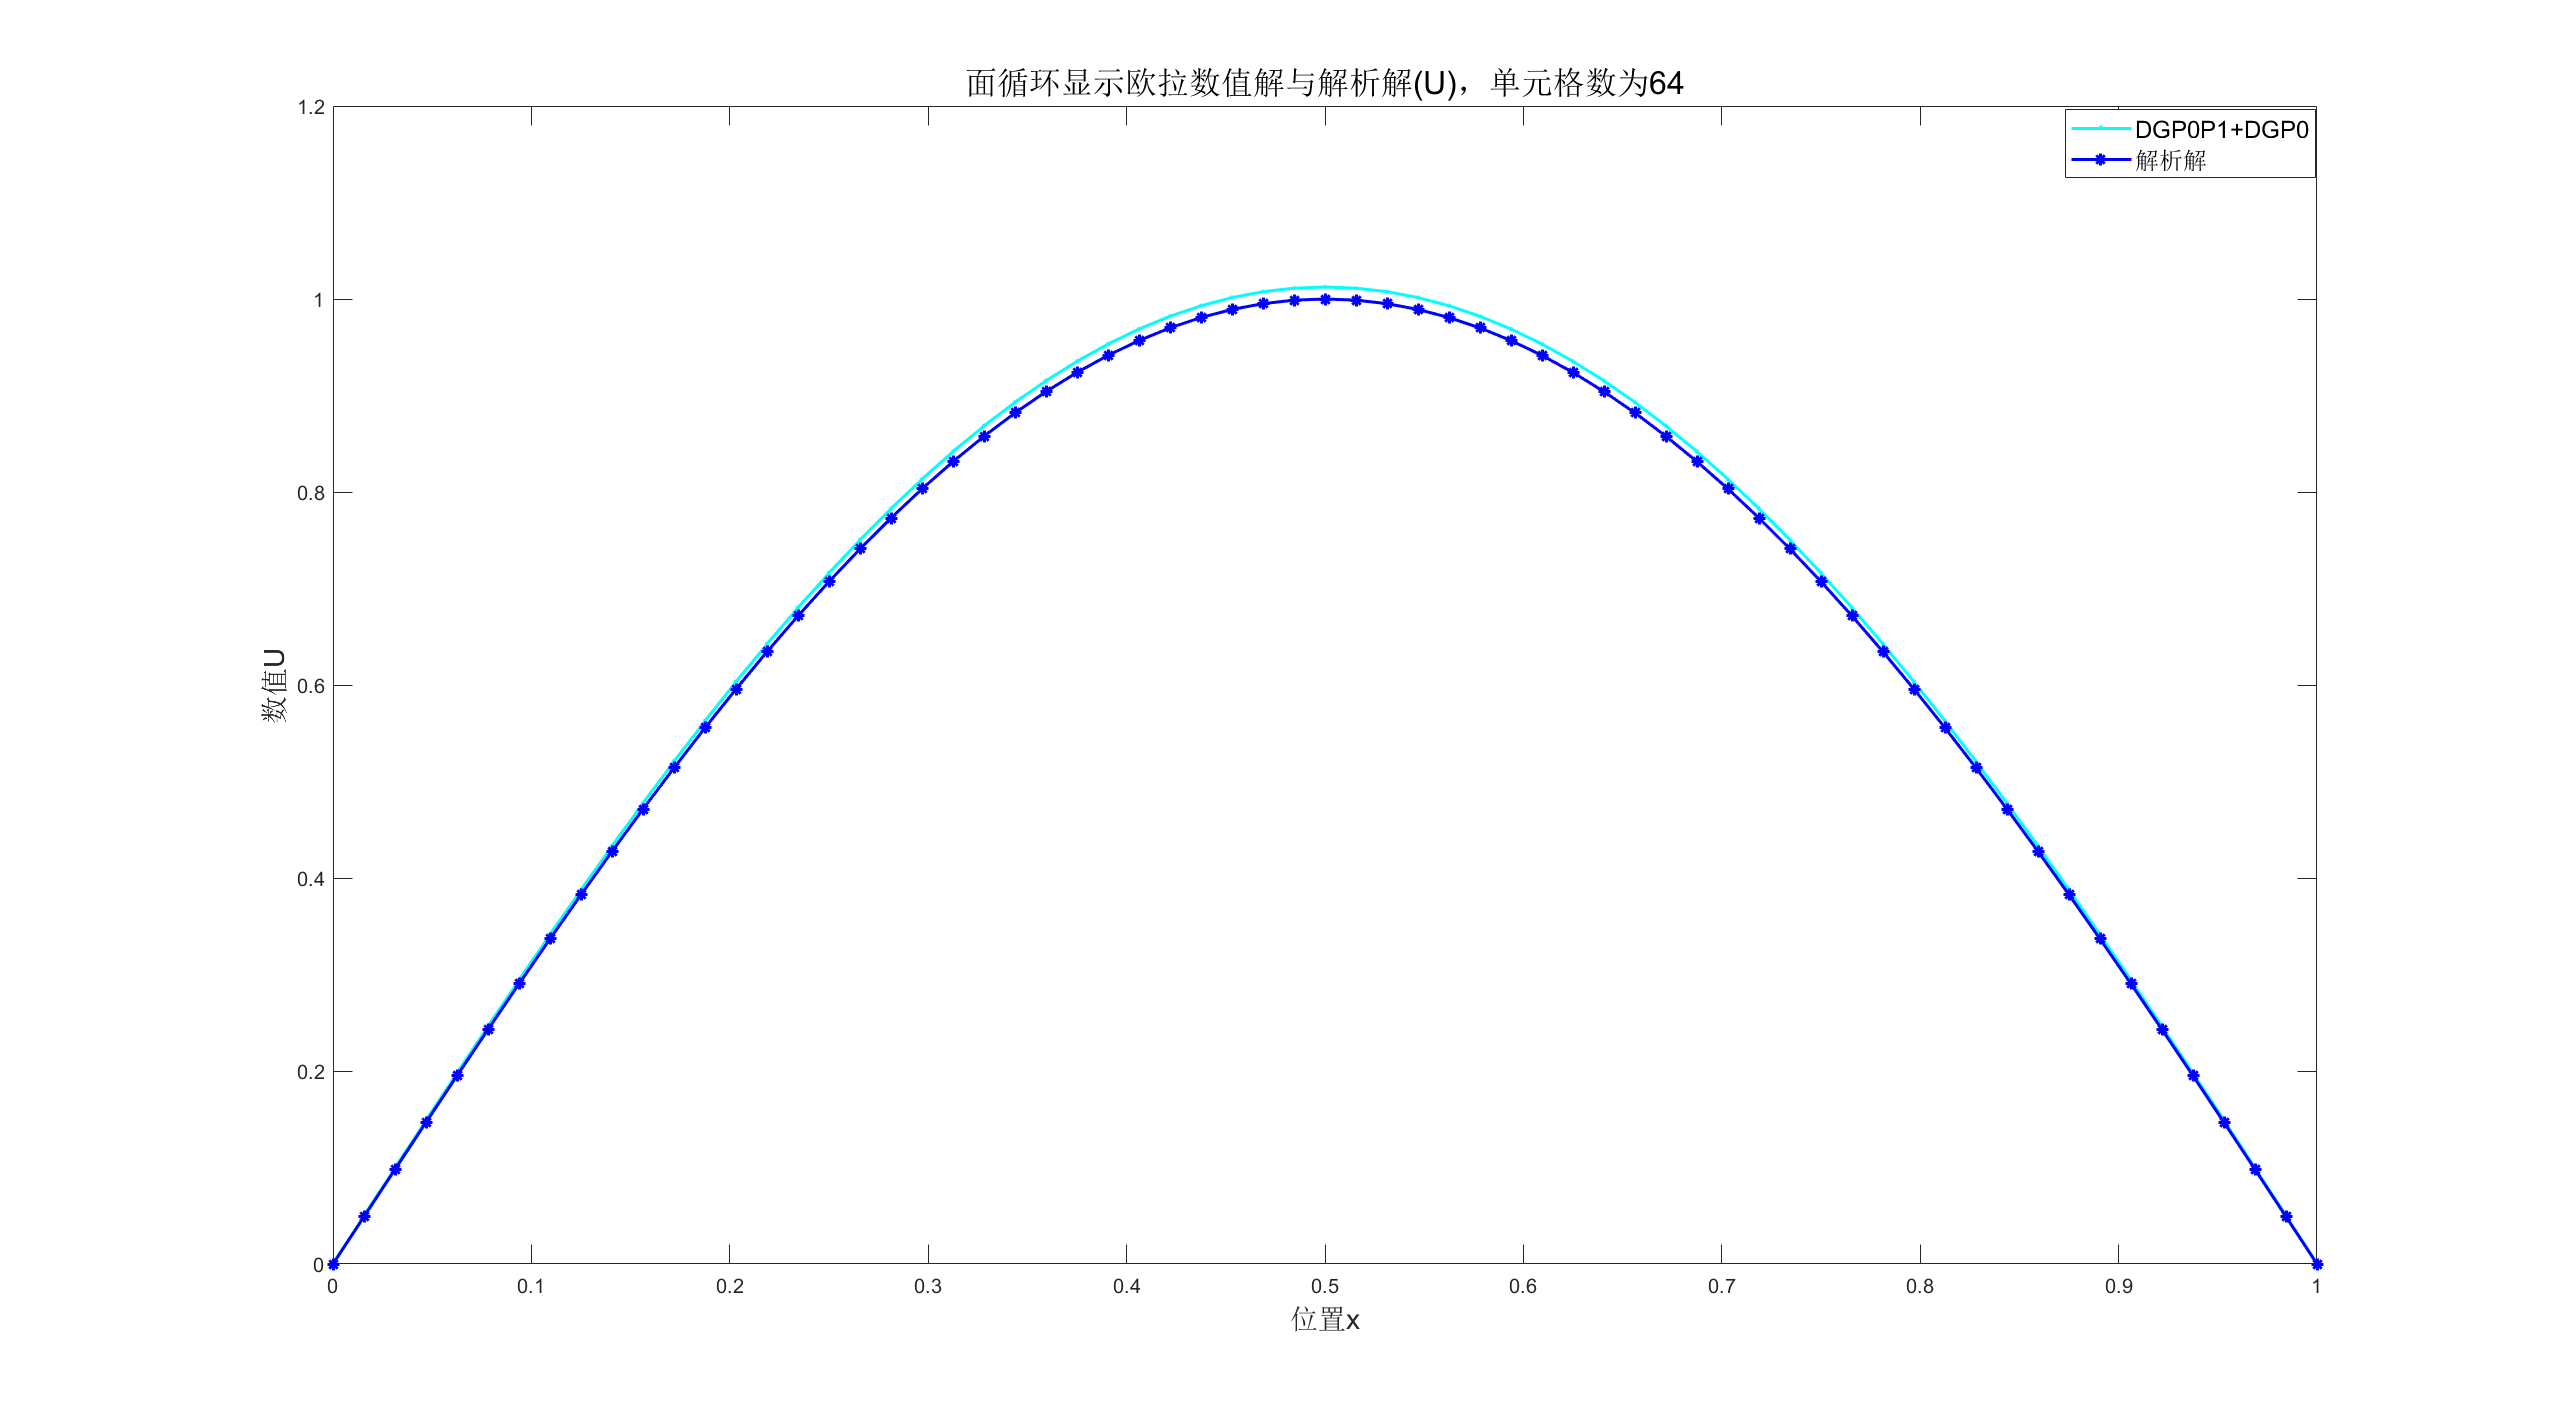
\includegraphics[width=3in]{obviouseuler/U64.png} }
		\caption{Explicit Euler U}
	\end{figure}\\
	
	\begin{figure}[!h]
		\centering
		\subfloat[8 elements]{
			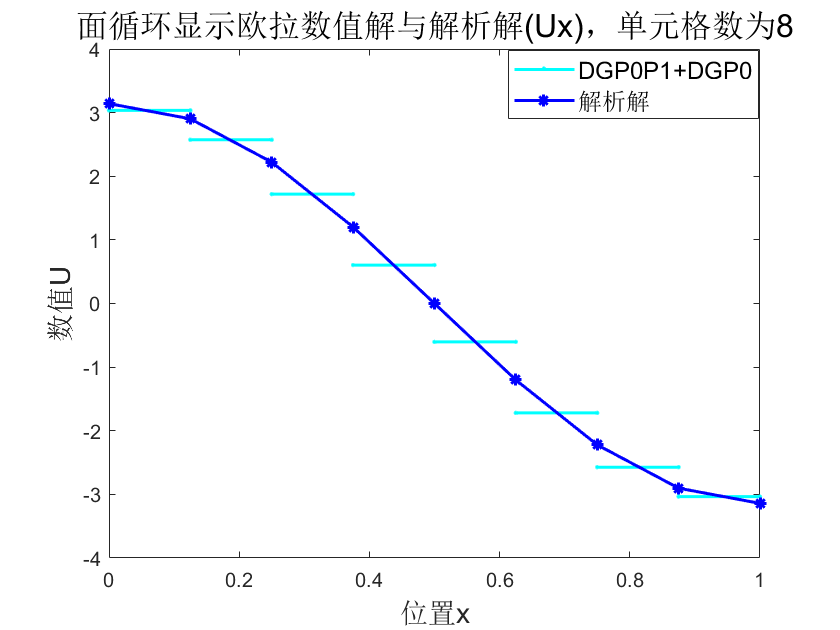
\includegraphics[width=3in]{obviouseuler/Ux8.png} 
		}
		\hfill
		\subfloat[64 elements]{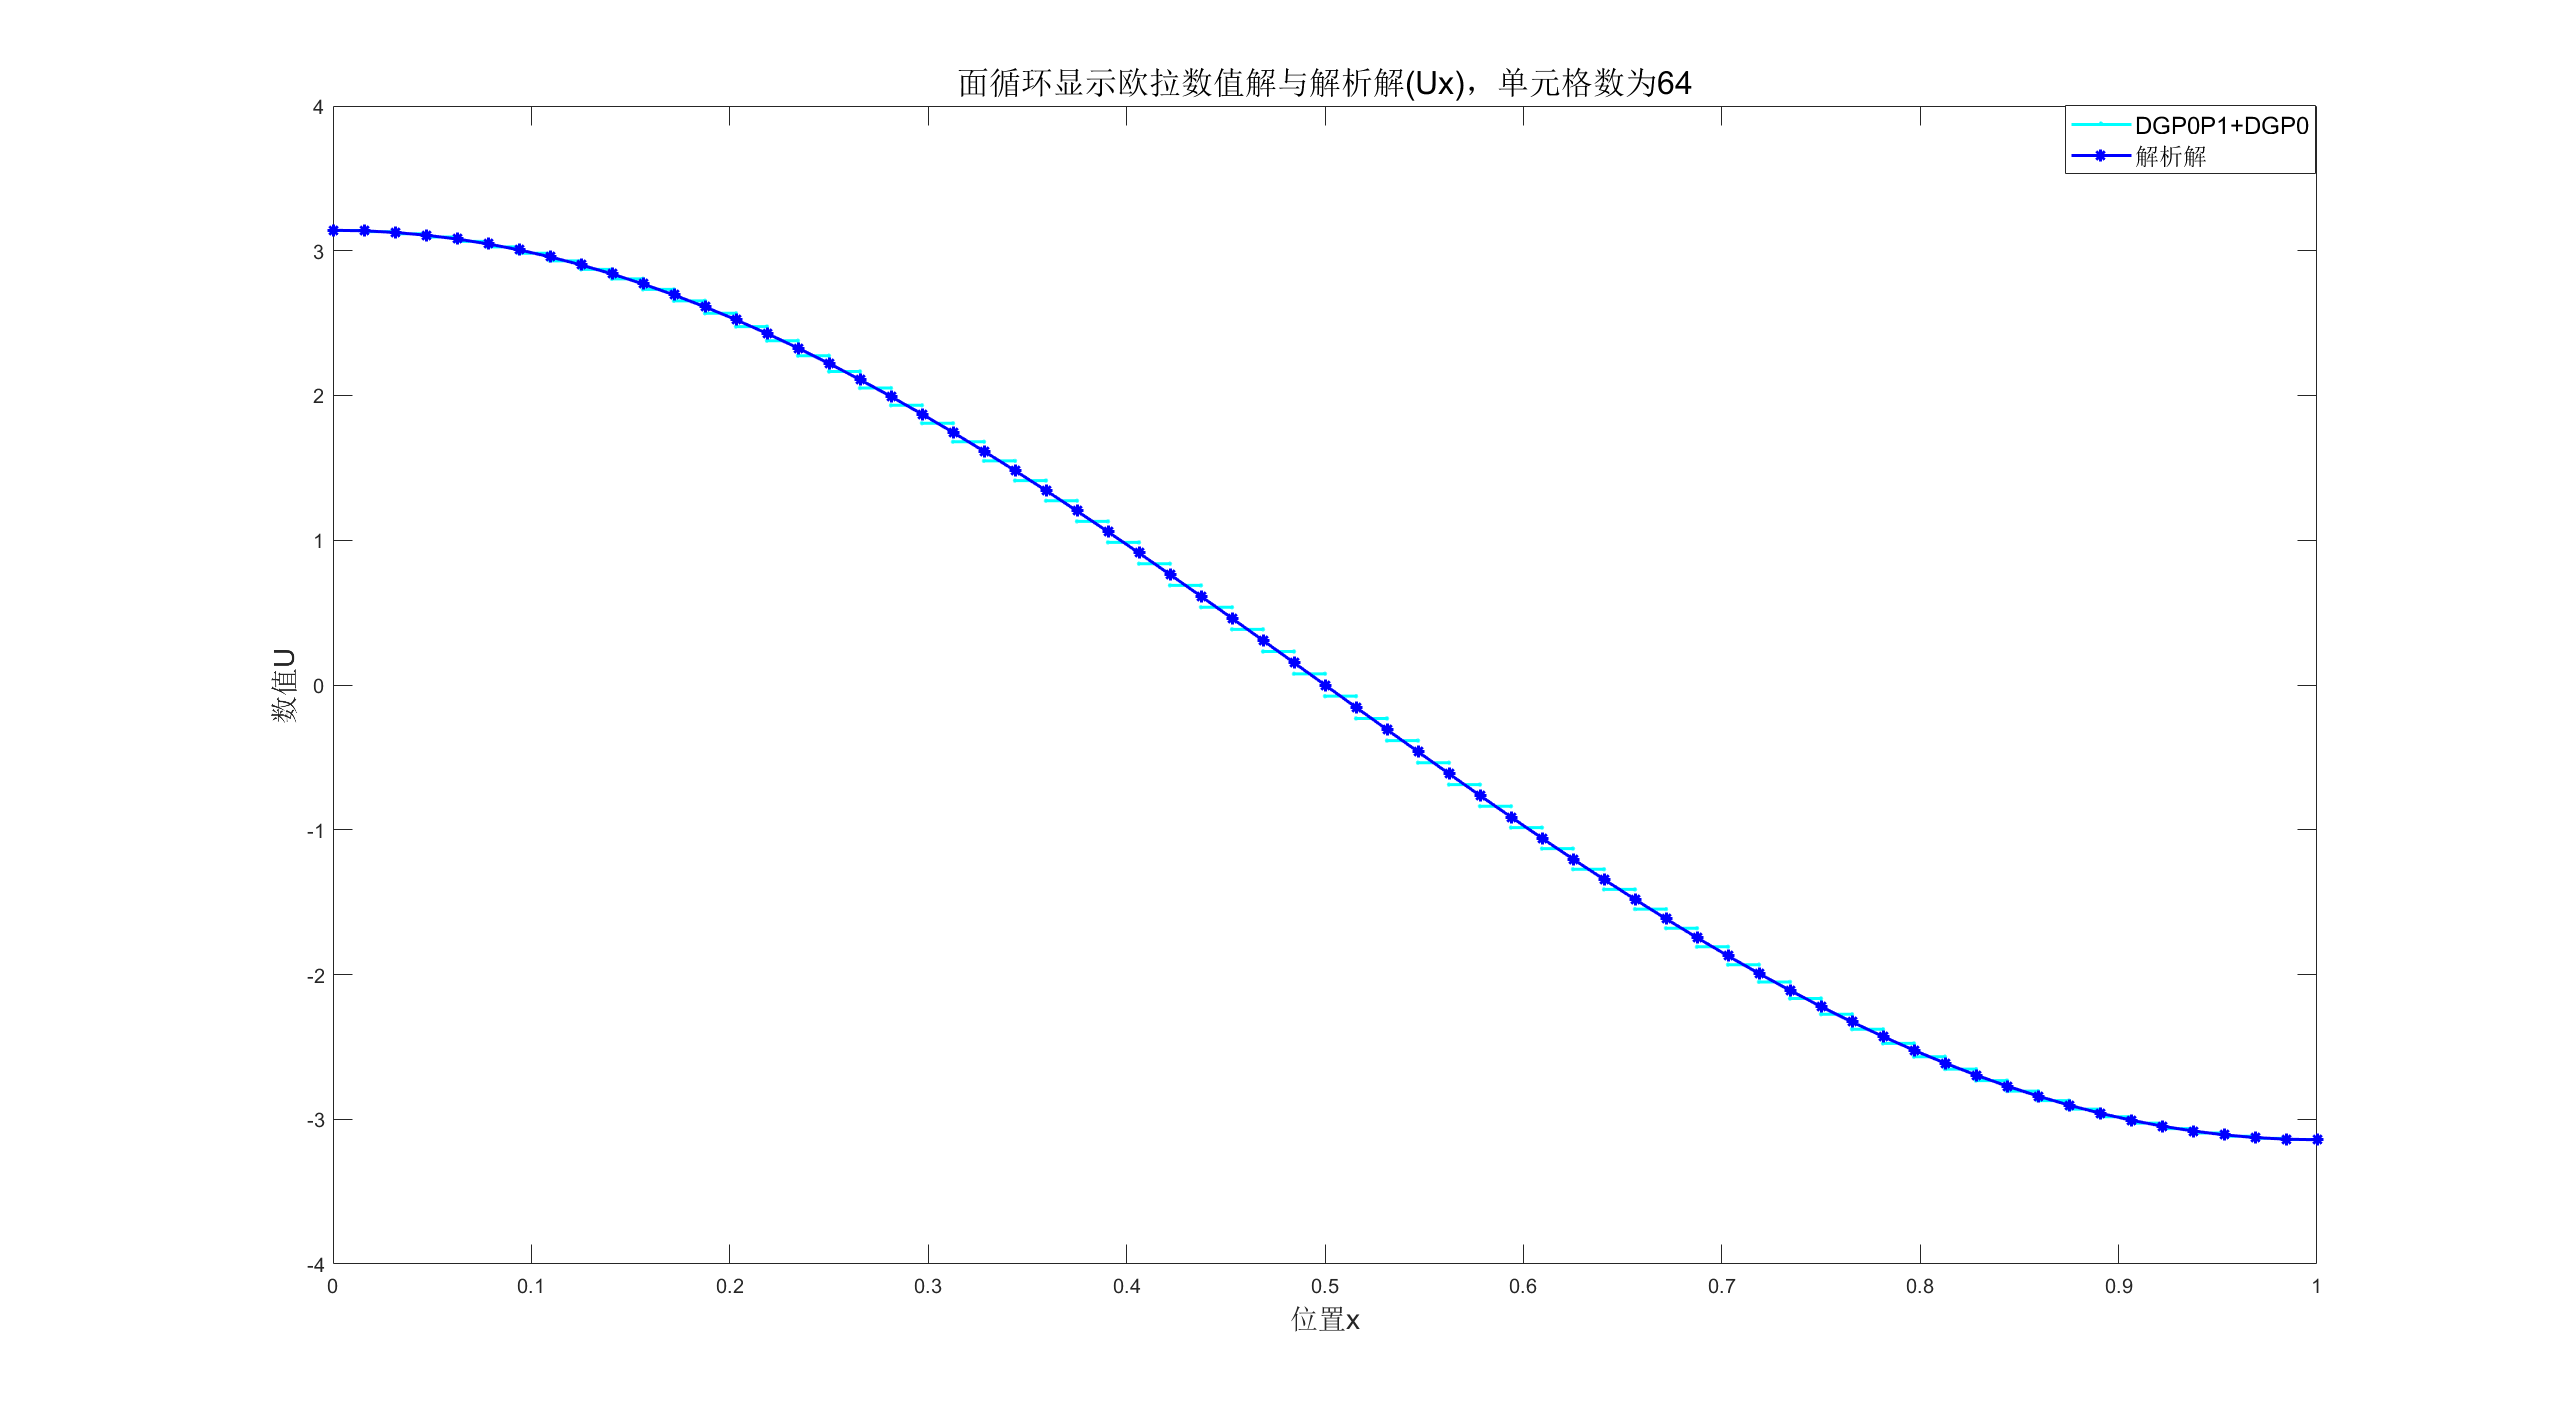
\includegraphics[width=3in]{obviouseuler/Ux64.png} }
		\caption{Explicit Euler Ux}
	\end{figure}\leavevmode\\

	\begin{figure}[!h]
	\centering
	\subfloat[U]{
		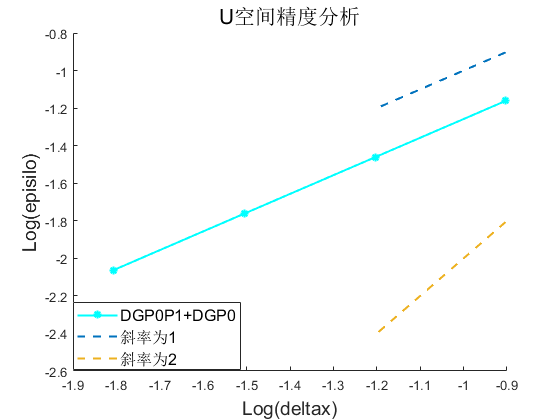
\includegraphics[width=3in]{obviouseuler/U空间精度分析.png} 
	}
	\hfill
	\subfloat[Ux]{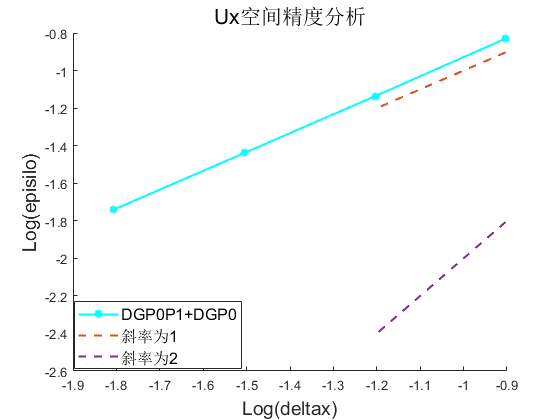
\includegraphics[width=3in]{obviouseuler/Ux空间精度分析.png} }
	\caption{空间精度}
\end{figure}\leavevmode\\

\clearpage
	B)\textbf{TVD-RK3}\\
\begin{figure}[!h]
	\centering
	\subfloat[8 elements]{
		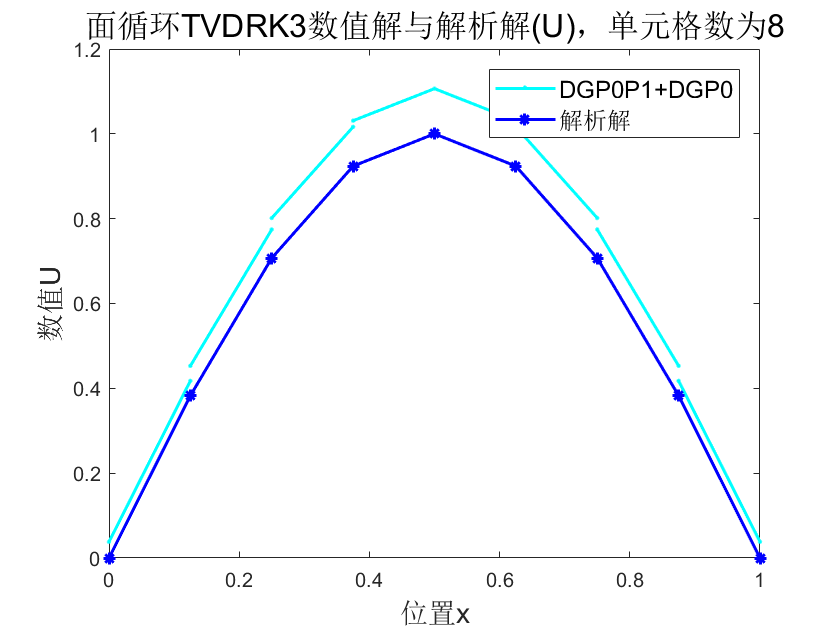
\includegraphics[width=3in]{TVDRK3/U8.png} 
	}
	\hfill
	\subfloat[64 elements]{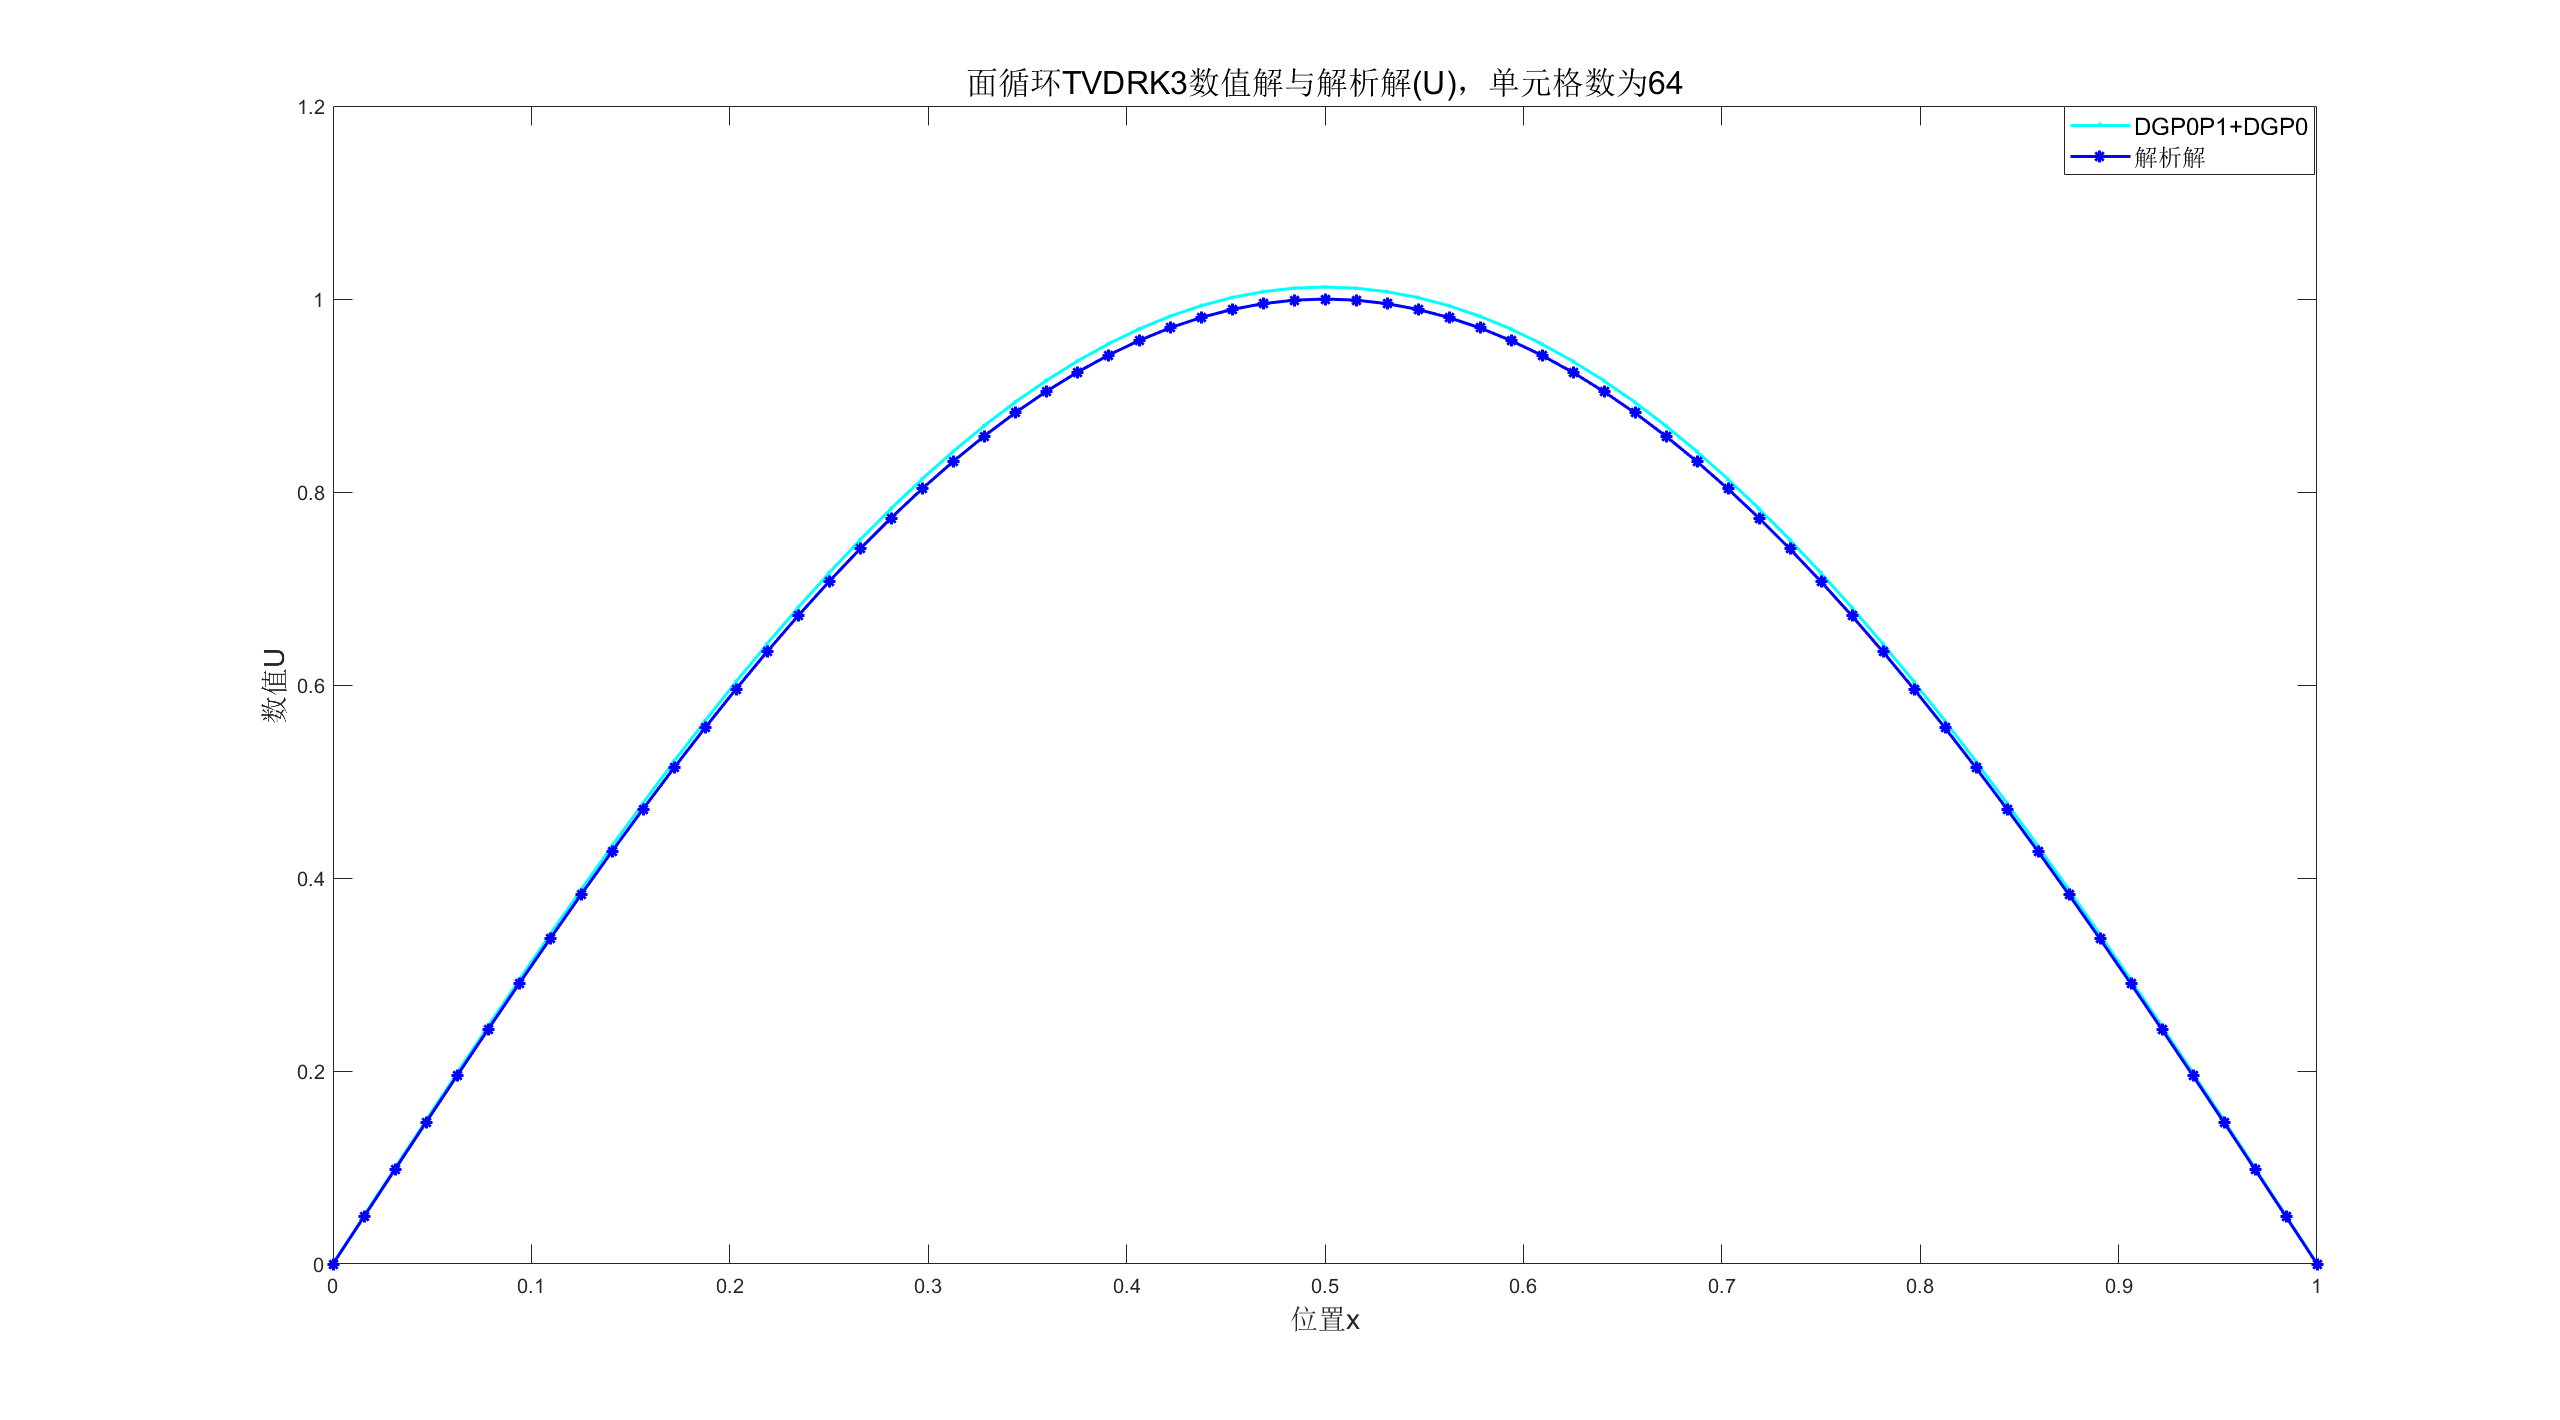
\includegraphics[width=3in]{TVDRK3/U64.png} }
	\caption{TVD-RK3 U}
\end{figure}\\


\begin{figure}[!h]
	\centering
	\subfloat[8 elements]{
		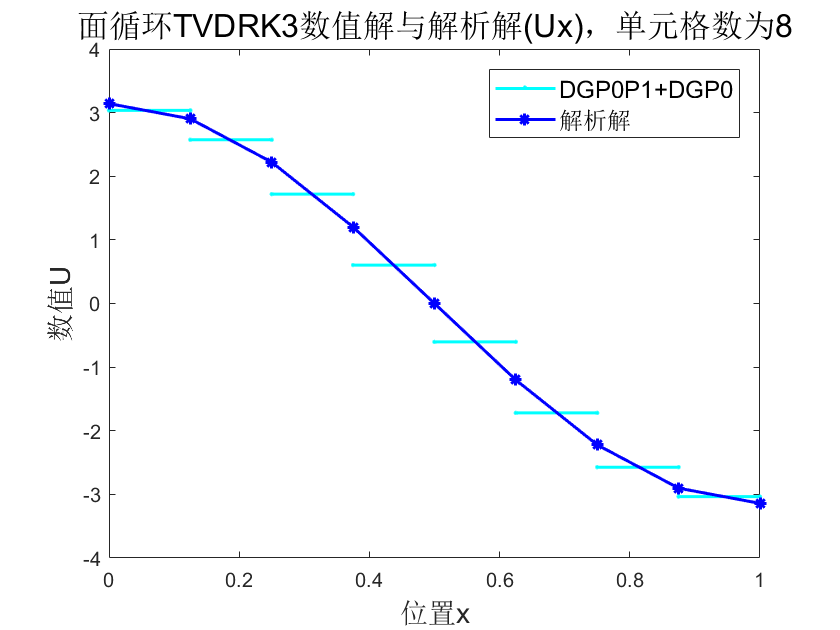
\includegraphics[width=3in]{TVDRK3/Ux8.png} 
	}
	\hfill
	\subfloat[64 elements]{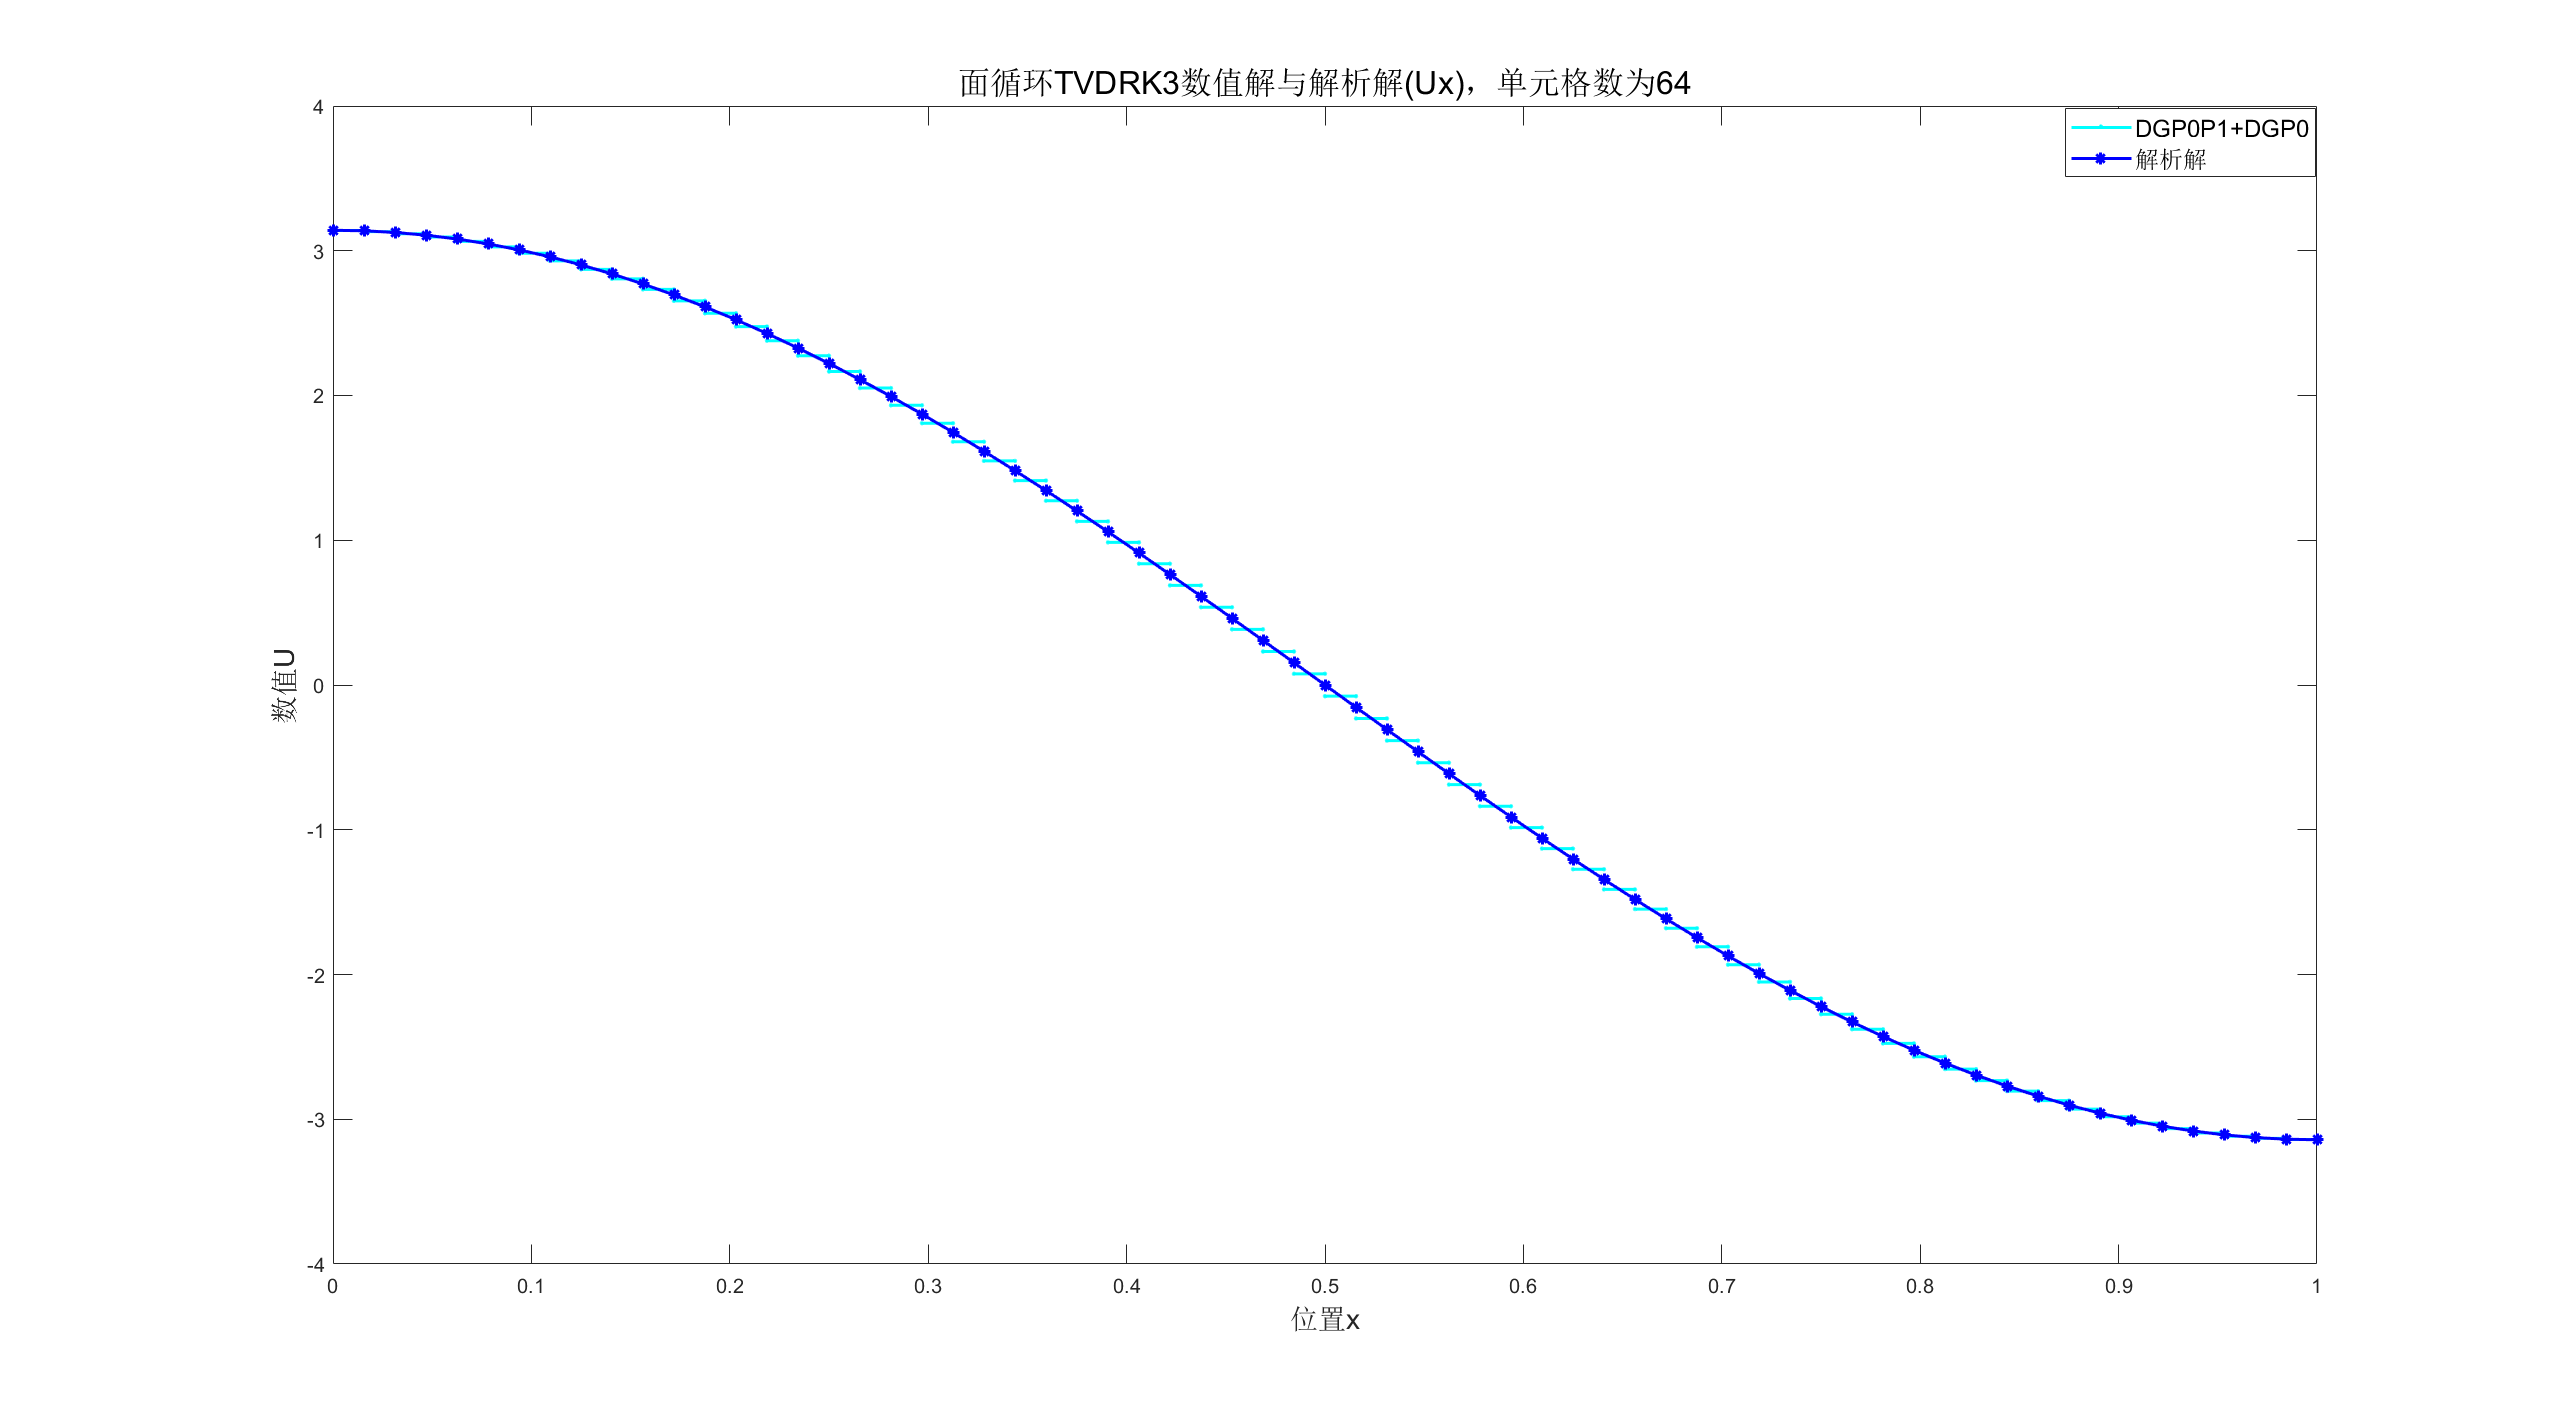
\includegraphics[width=3in]{TVDRK3/Ux64.png} }
	\caption{TVD-RK3 Ux}
\end{figure}\leavevmode\\

\begin{figure}[!h]
	\centering
	\subfloat[U]{
		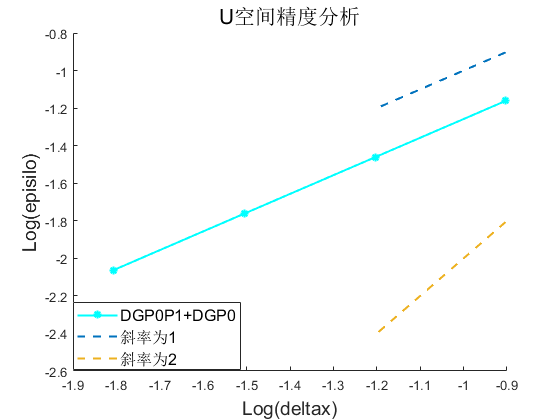
\includegraphics[width=3in]{TVDRK3/U空间精度.png} 
	}
	\hfill
	\subfloat[Ux]{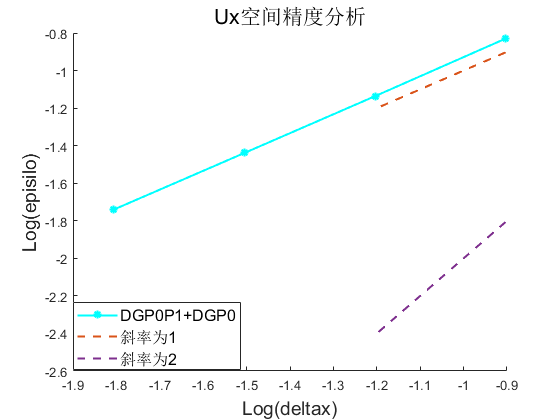
\includegraphics[width=3in]{TVDRK3/Ux空间精度.png} }
	\caption{空间精度}
\end{figure}\leavevmode\\

\clearpage
C)\textbf{BDF1}\\
\begin{figure}[!h]
	\centering
	\subfloat[8 elements]{
		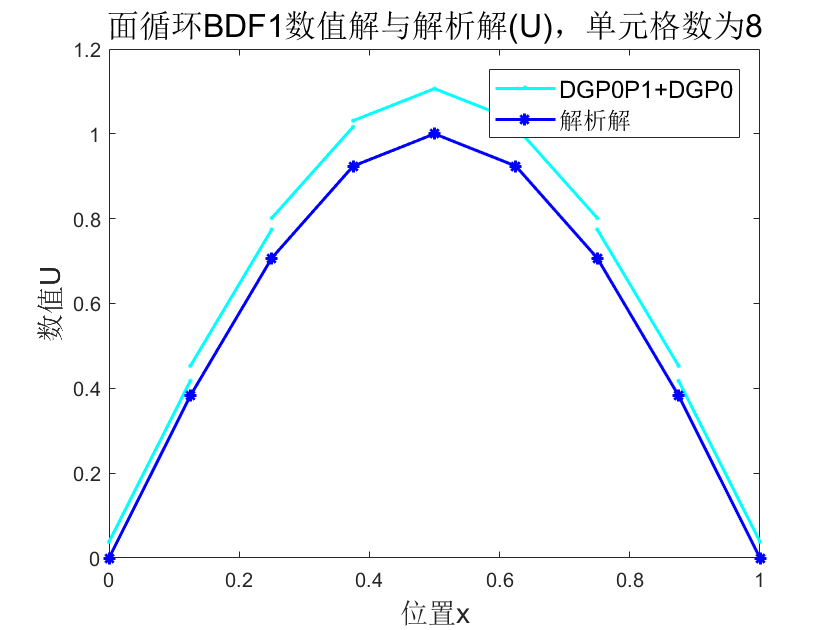
\includegraphics[width=3in]{BDF1/U8.png} 
	}
	\hfill
	\subfloat[64 elements]{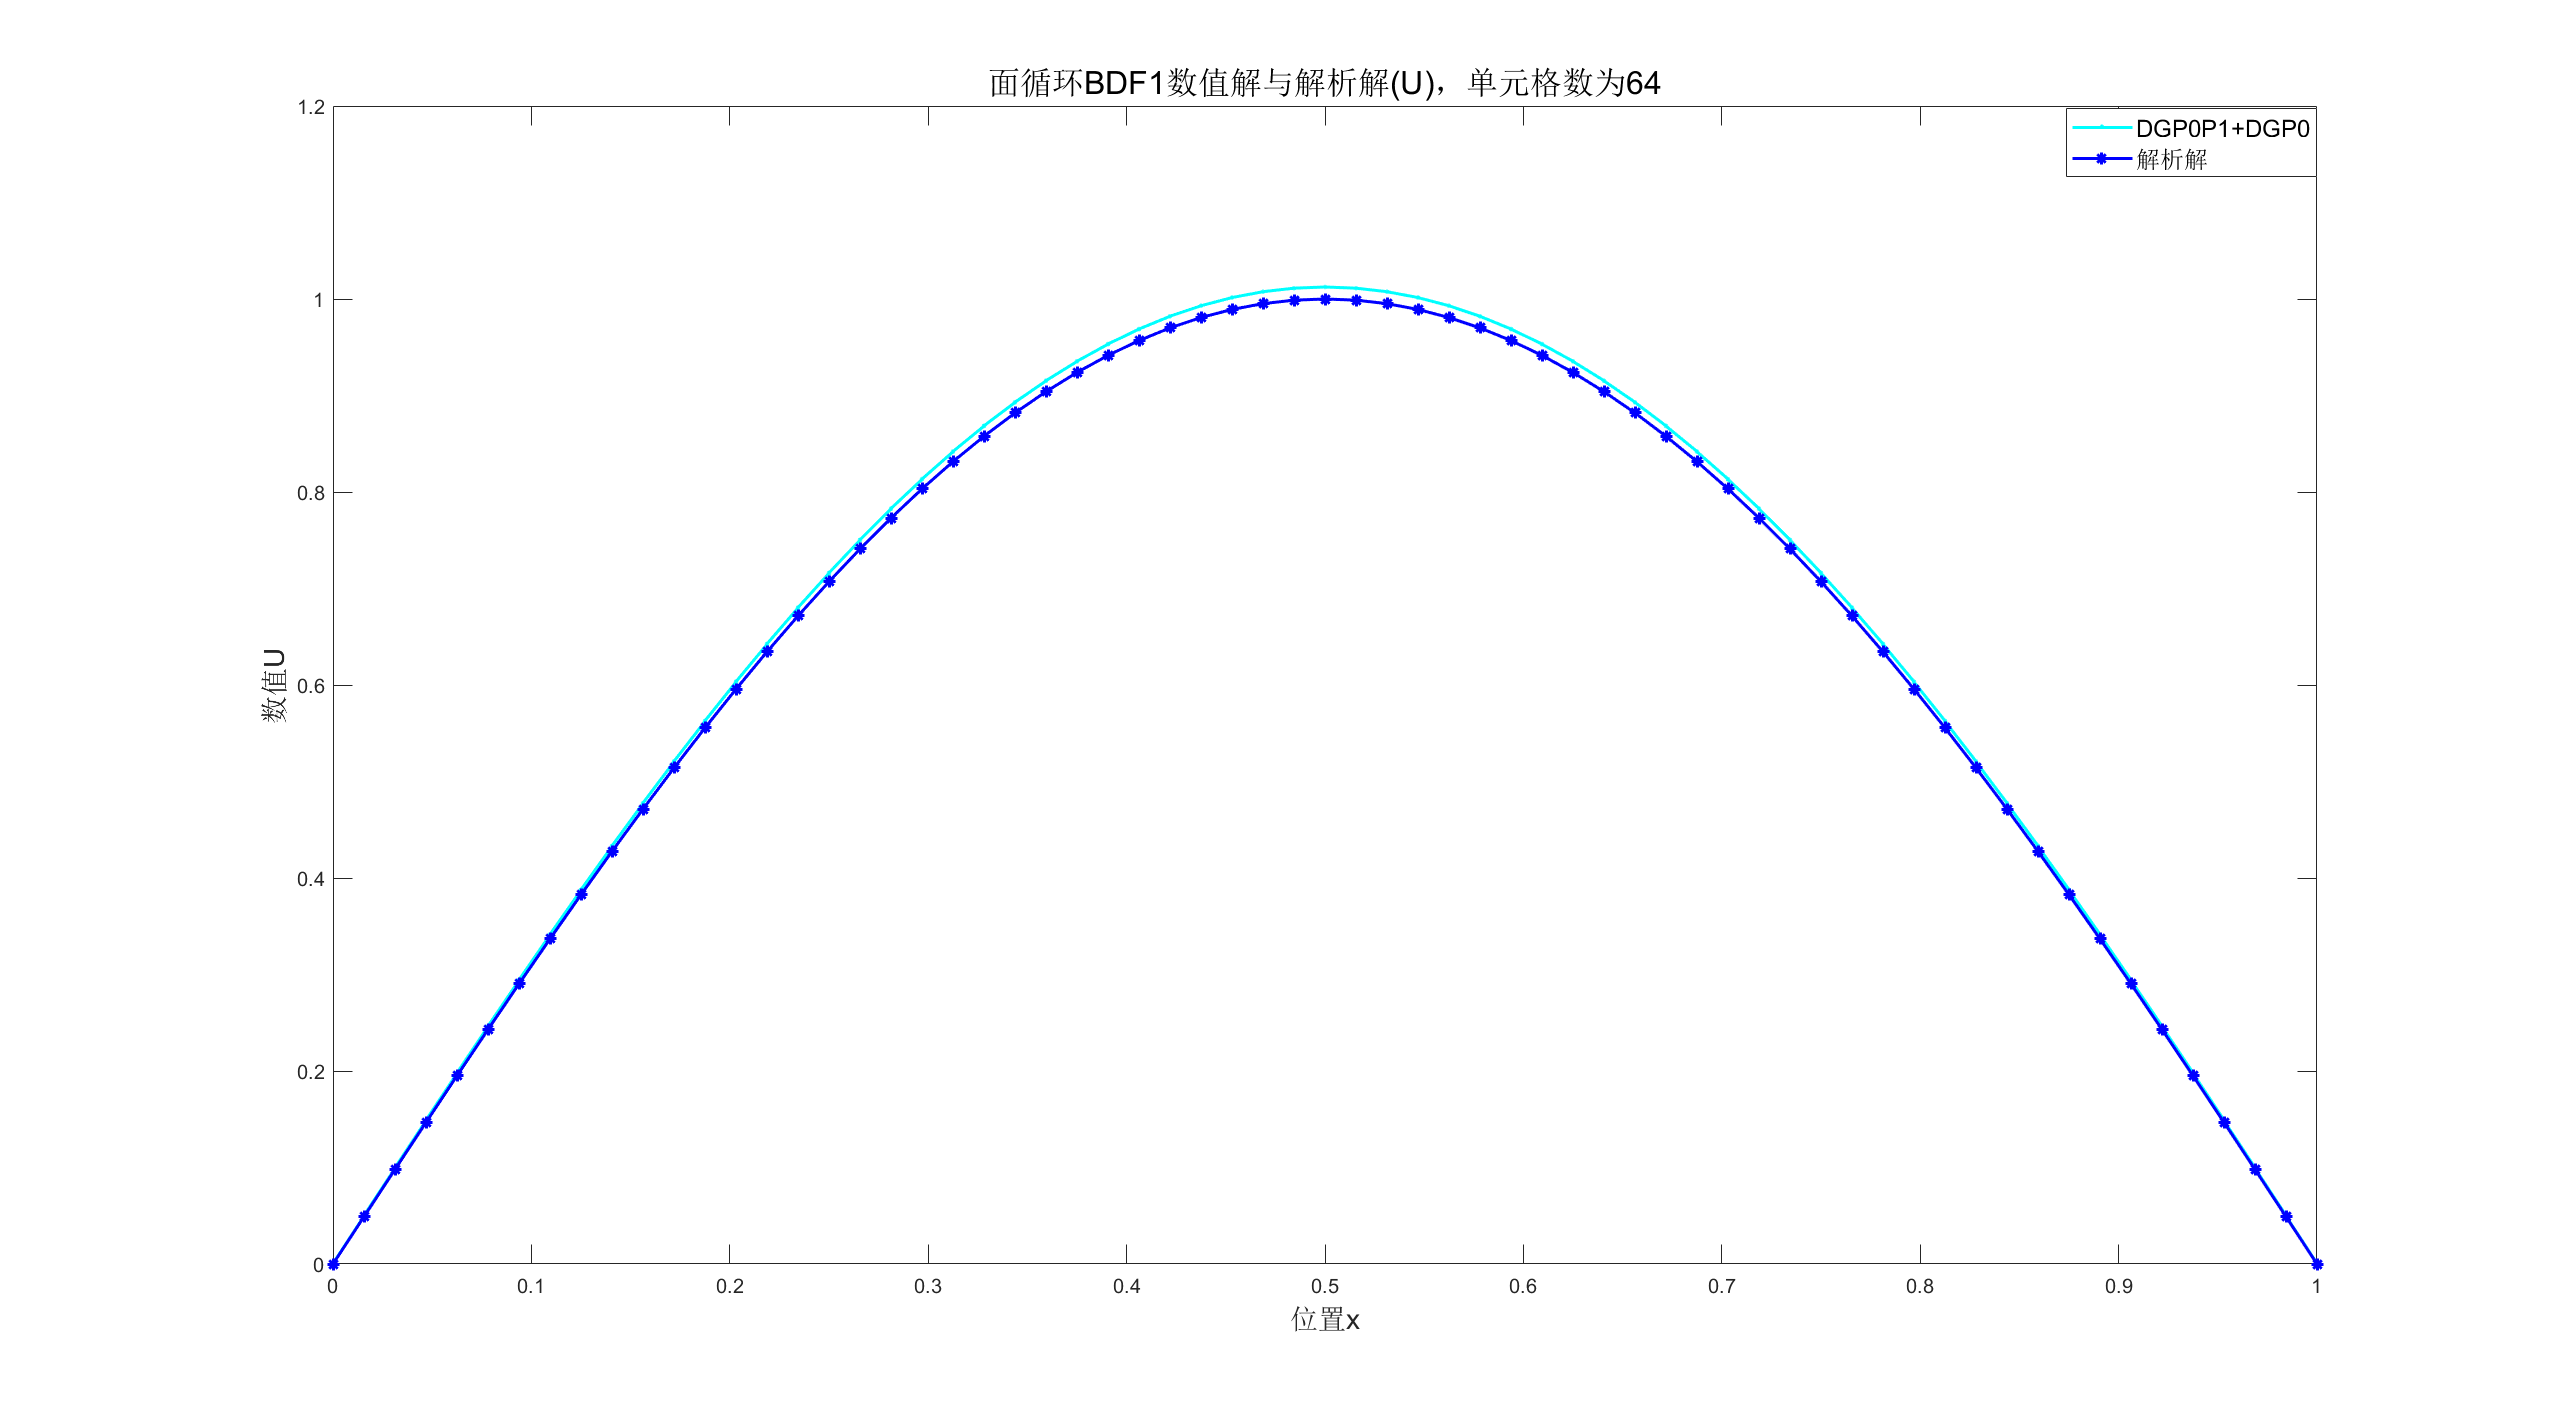
\includegraphics[width=3in]{BDF1/U64.png} }
	\caption{BDF1 U}
\end{figure}\\


\begin{figure}[!h]
	\centering
	\subfloat[8 elements]{
		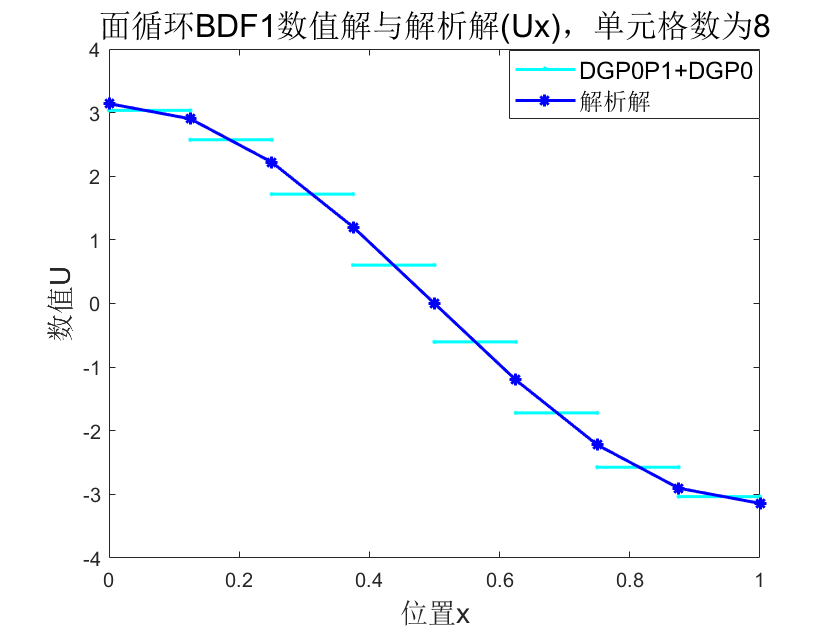
\includegraphics[width=3in]{BDF1/Ux8.png} 
	}
	\hfill
	\subfloat[64 elements]{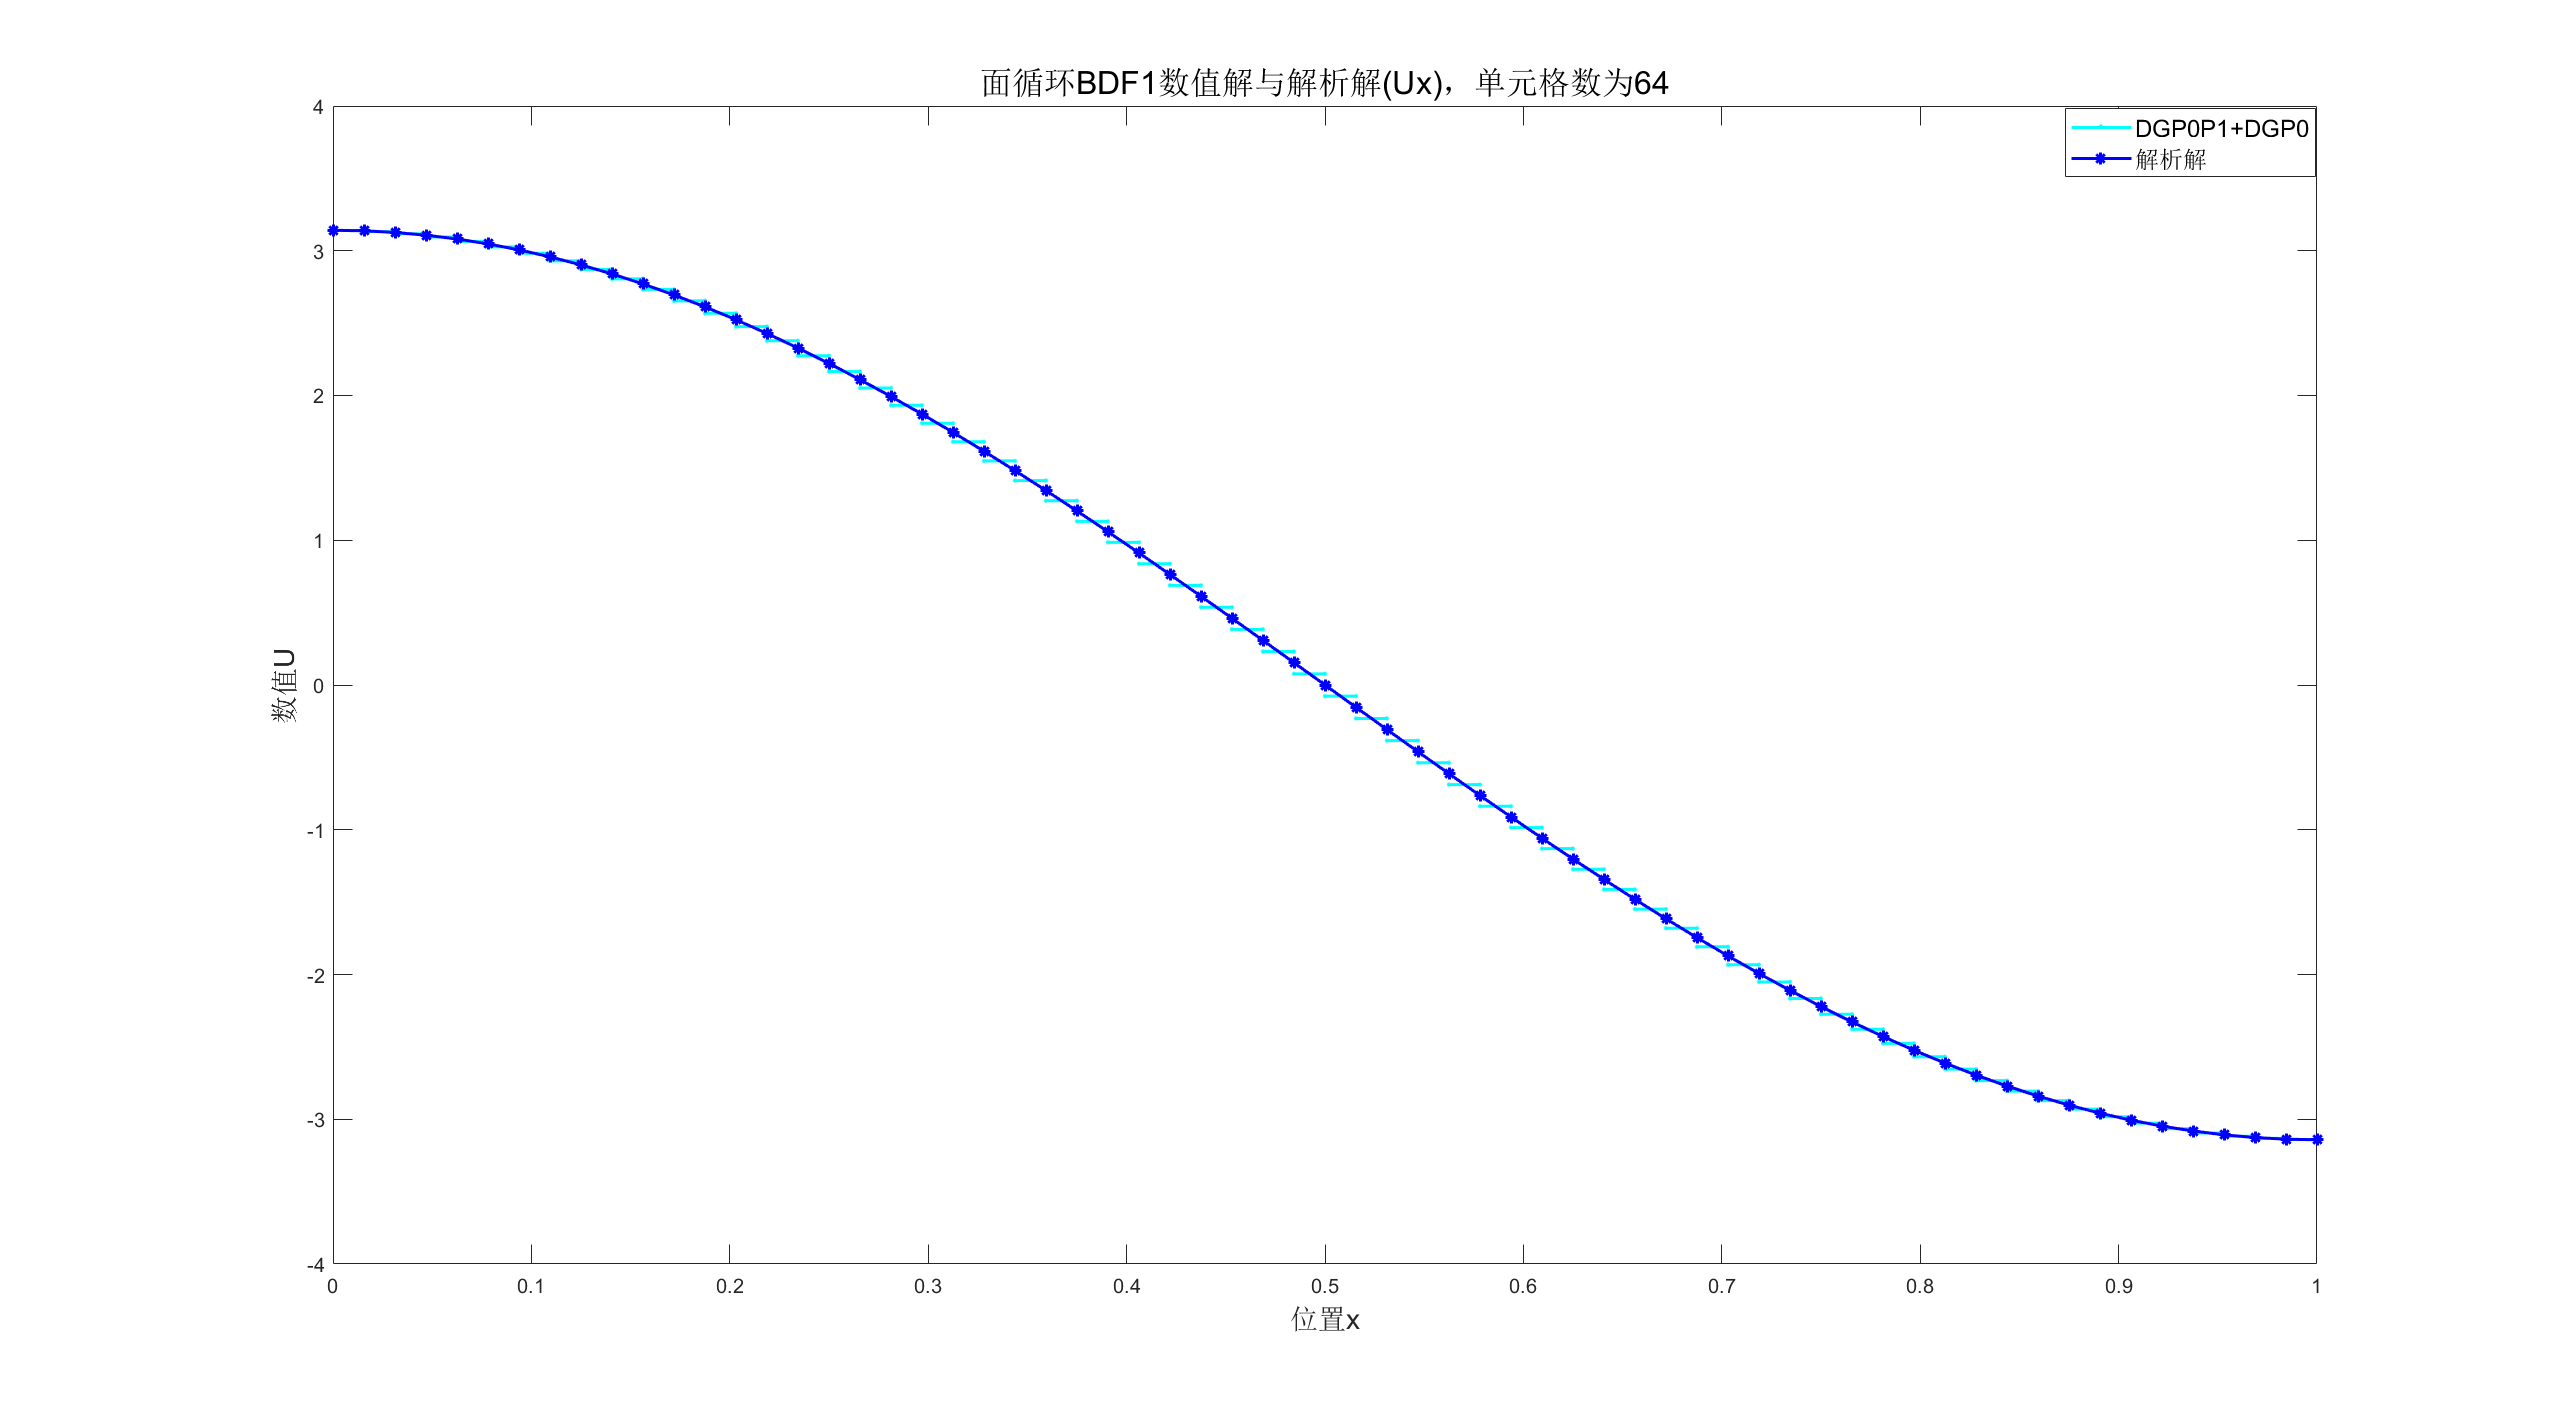
\includegraphics[width=3in]{BDF1/Ux64.png} }
	\caption{BDF1 Ux}
\end{figure}\leavevmode\\

\begin{figure}[!h]
	\centering
	\subfloat[U]{
		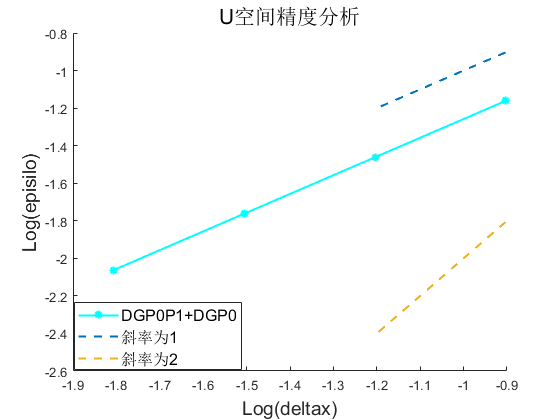
\includegraphics[width=3in]{BDF1/U空间精度分析.png} 
	}
	\hfill
	\subfloat[Ux]{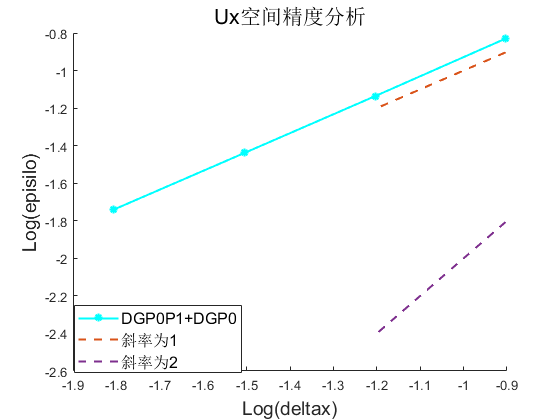
\includegraphics[width=3in]{BDF1/Ux空间精度分析.png} }
	\caption{空间精度}
\end{figure}\leavevmode\\
\clearpage
\textbf{解:}\\
\indent(2)生成网格时对网格点进行扰动,这会影响$\Delta x$,进而会影响到每个单元上的$\Delta \tau$,这里采用了两种向前推进方法:a)取所有单元的最小$\Delta \tau$进行推进(如下面的TVD-RK3),b)每个单元取自己对应的$\Delta \tau$,最后终止的$End \tau$取最大的那个(如下面的Obvious Euler和BDF1)。\\
\indent 以下展示非均匀网格下三种时间离散格式下(单元格数为8,64)的方程数值解与解析解对比图以及空间精度(这里仍然采取的均匀网格的$\Delta x$),结果显示两种推进方式得到的U的精度相似,但方法b)得到的Ux精度较好。\\

A)\textbf{Nonuniform grid explicit euler}\\
\begin{figure}[!h]
	\centering
	\subfloat[8 elements]{
		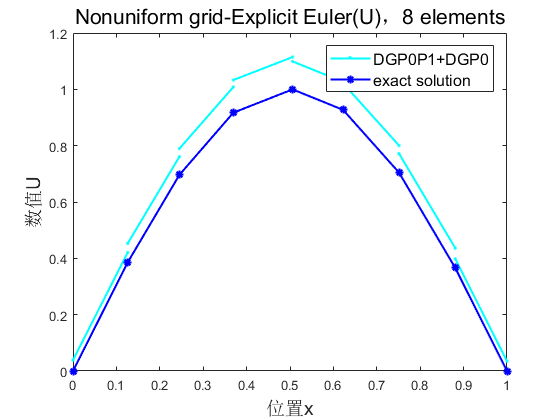
\includegraphics[width=3in]{ununiform grid obviouseuler/U8.png} 
	}
	\hfill
	\subfloat[64 elements]{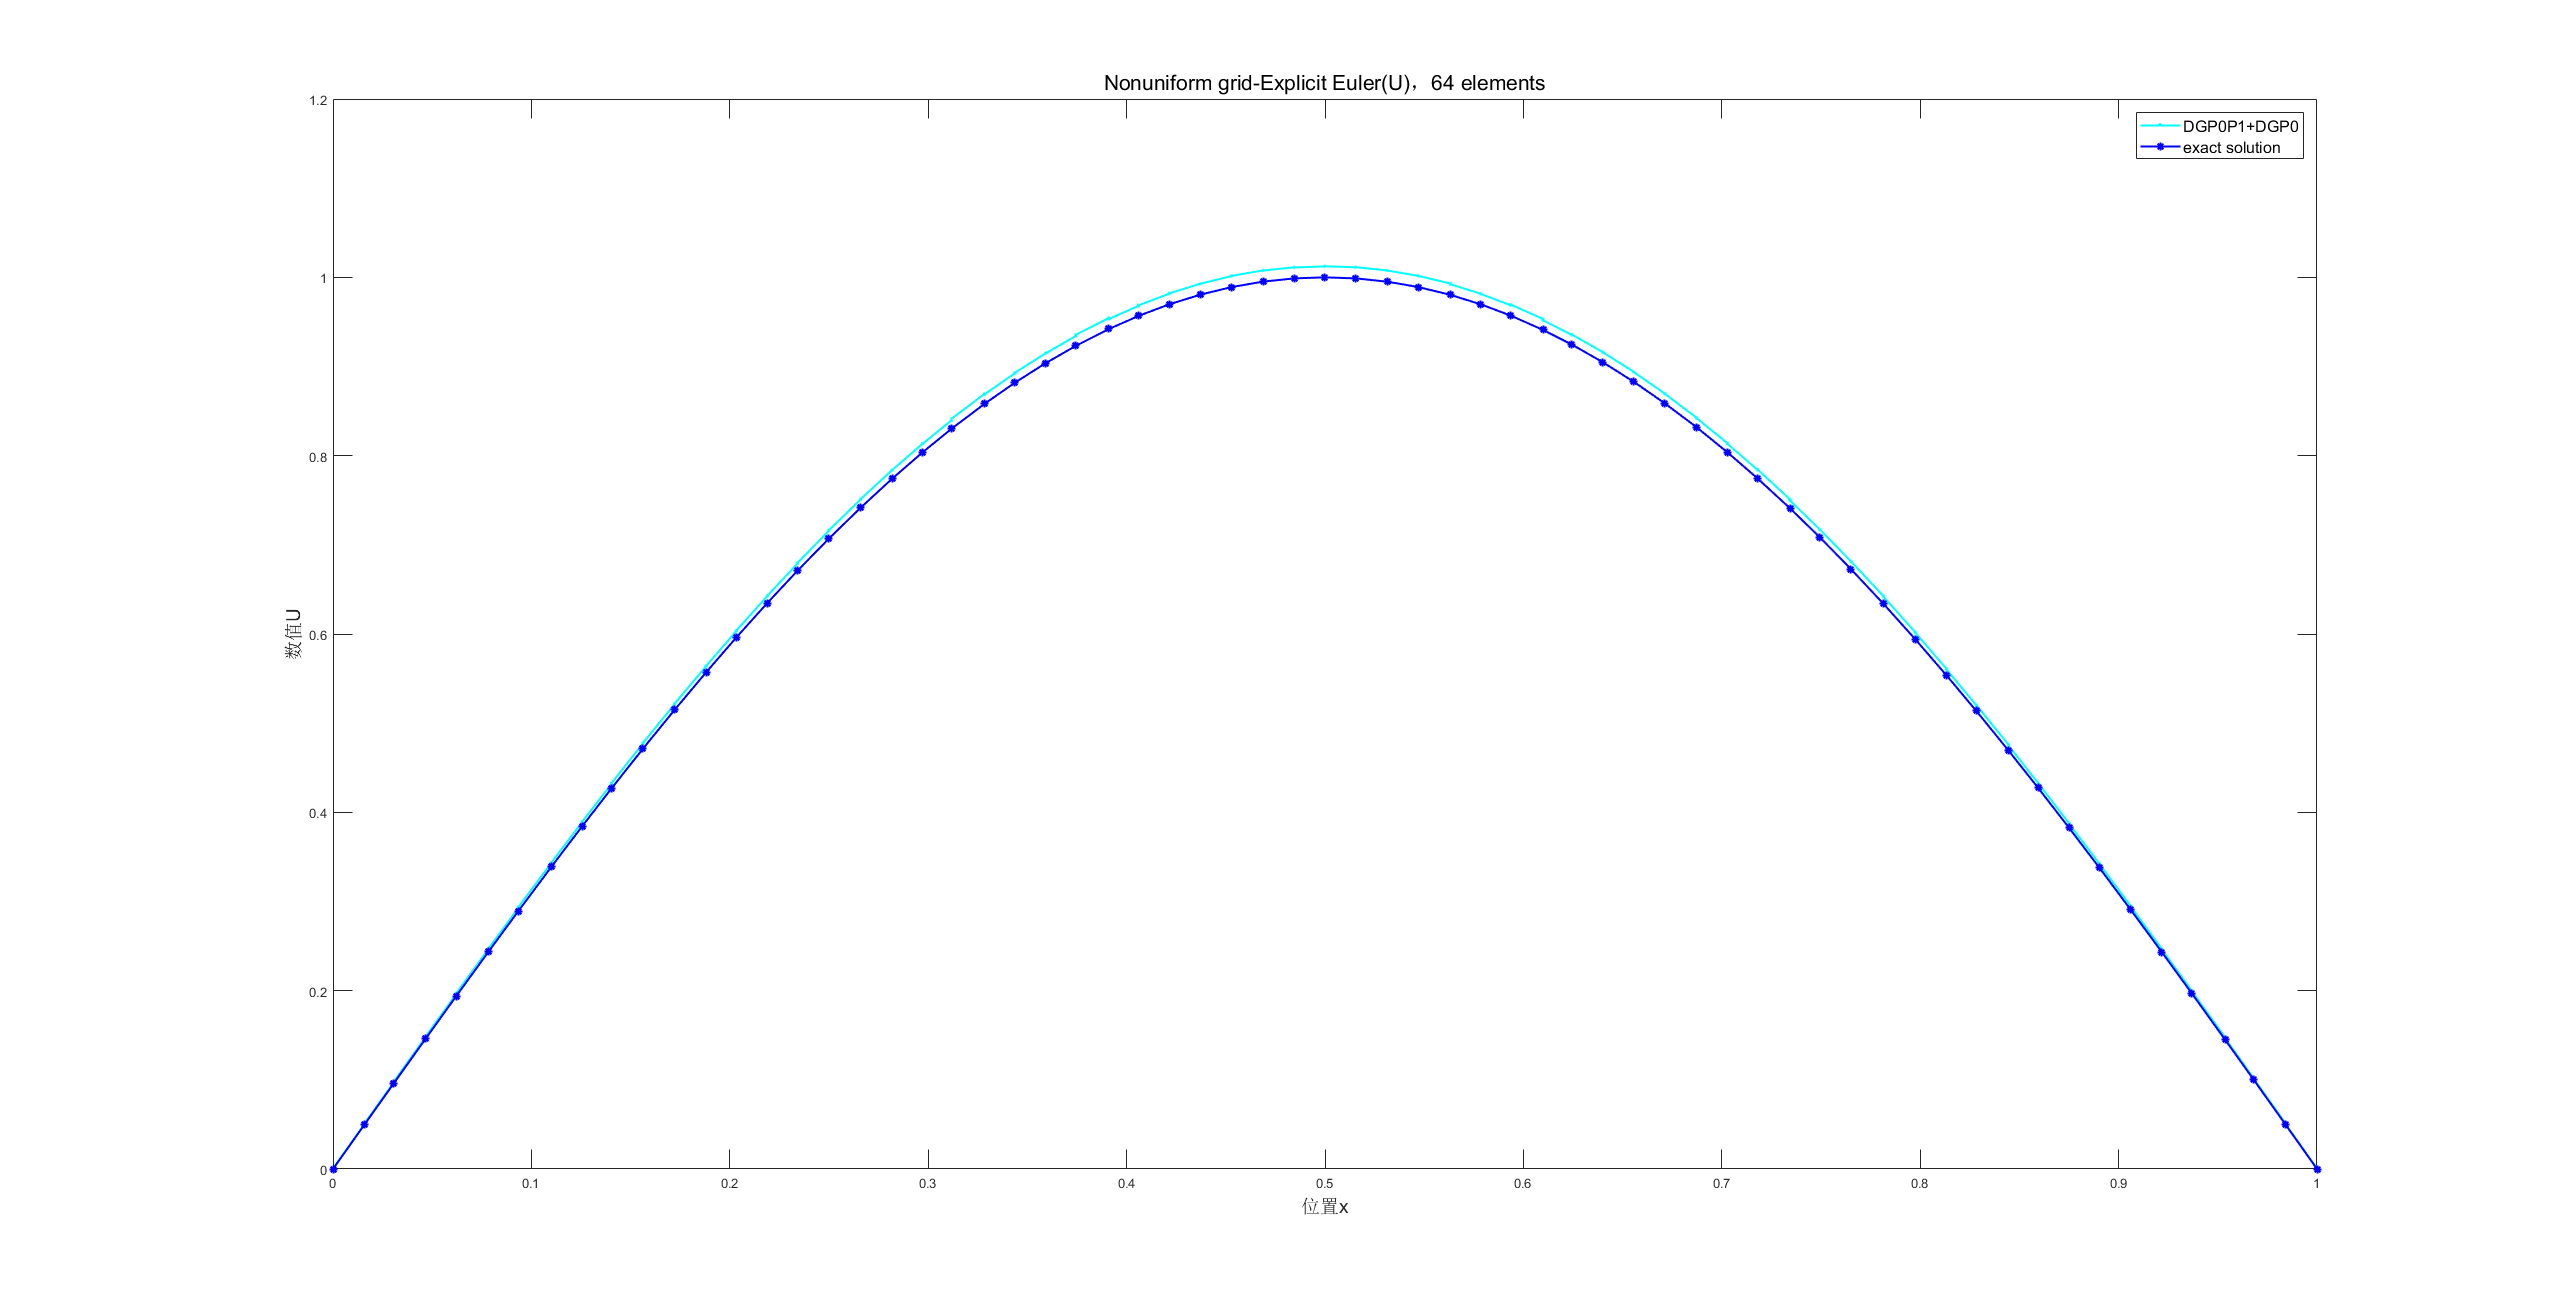
\includegraphics[width=3in]{ununiform grid obviouseuler/U64.png} }
	\caption{Nonuniform grid Explicit euler U}
\end{figure}\\


\begin{figure}[!h]
	\centering
	\subfloat[8 elements]{
		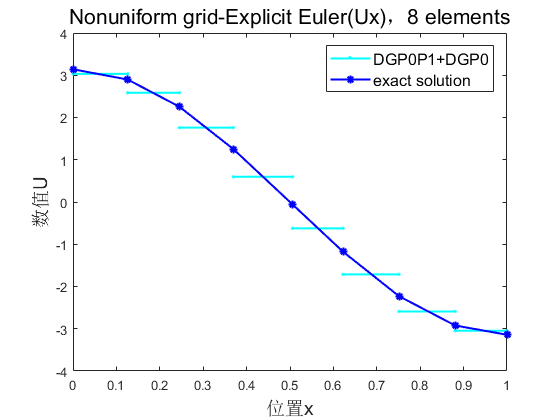
\includegraphics[width=3in]{ununiform grid obviouseuler/Ux8.png} 
	}
	\hfill
	\subfloat[64 elements]{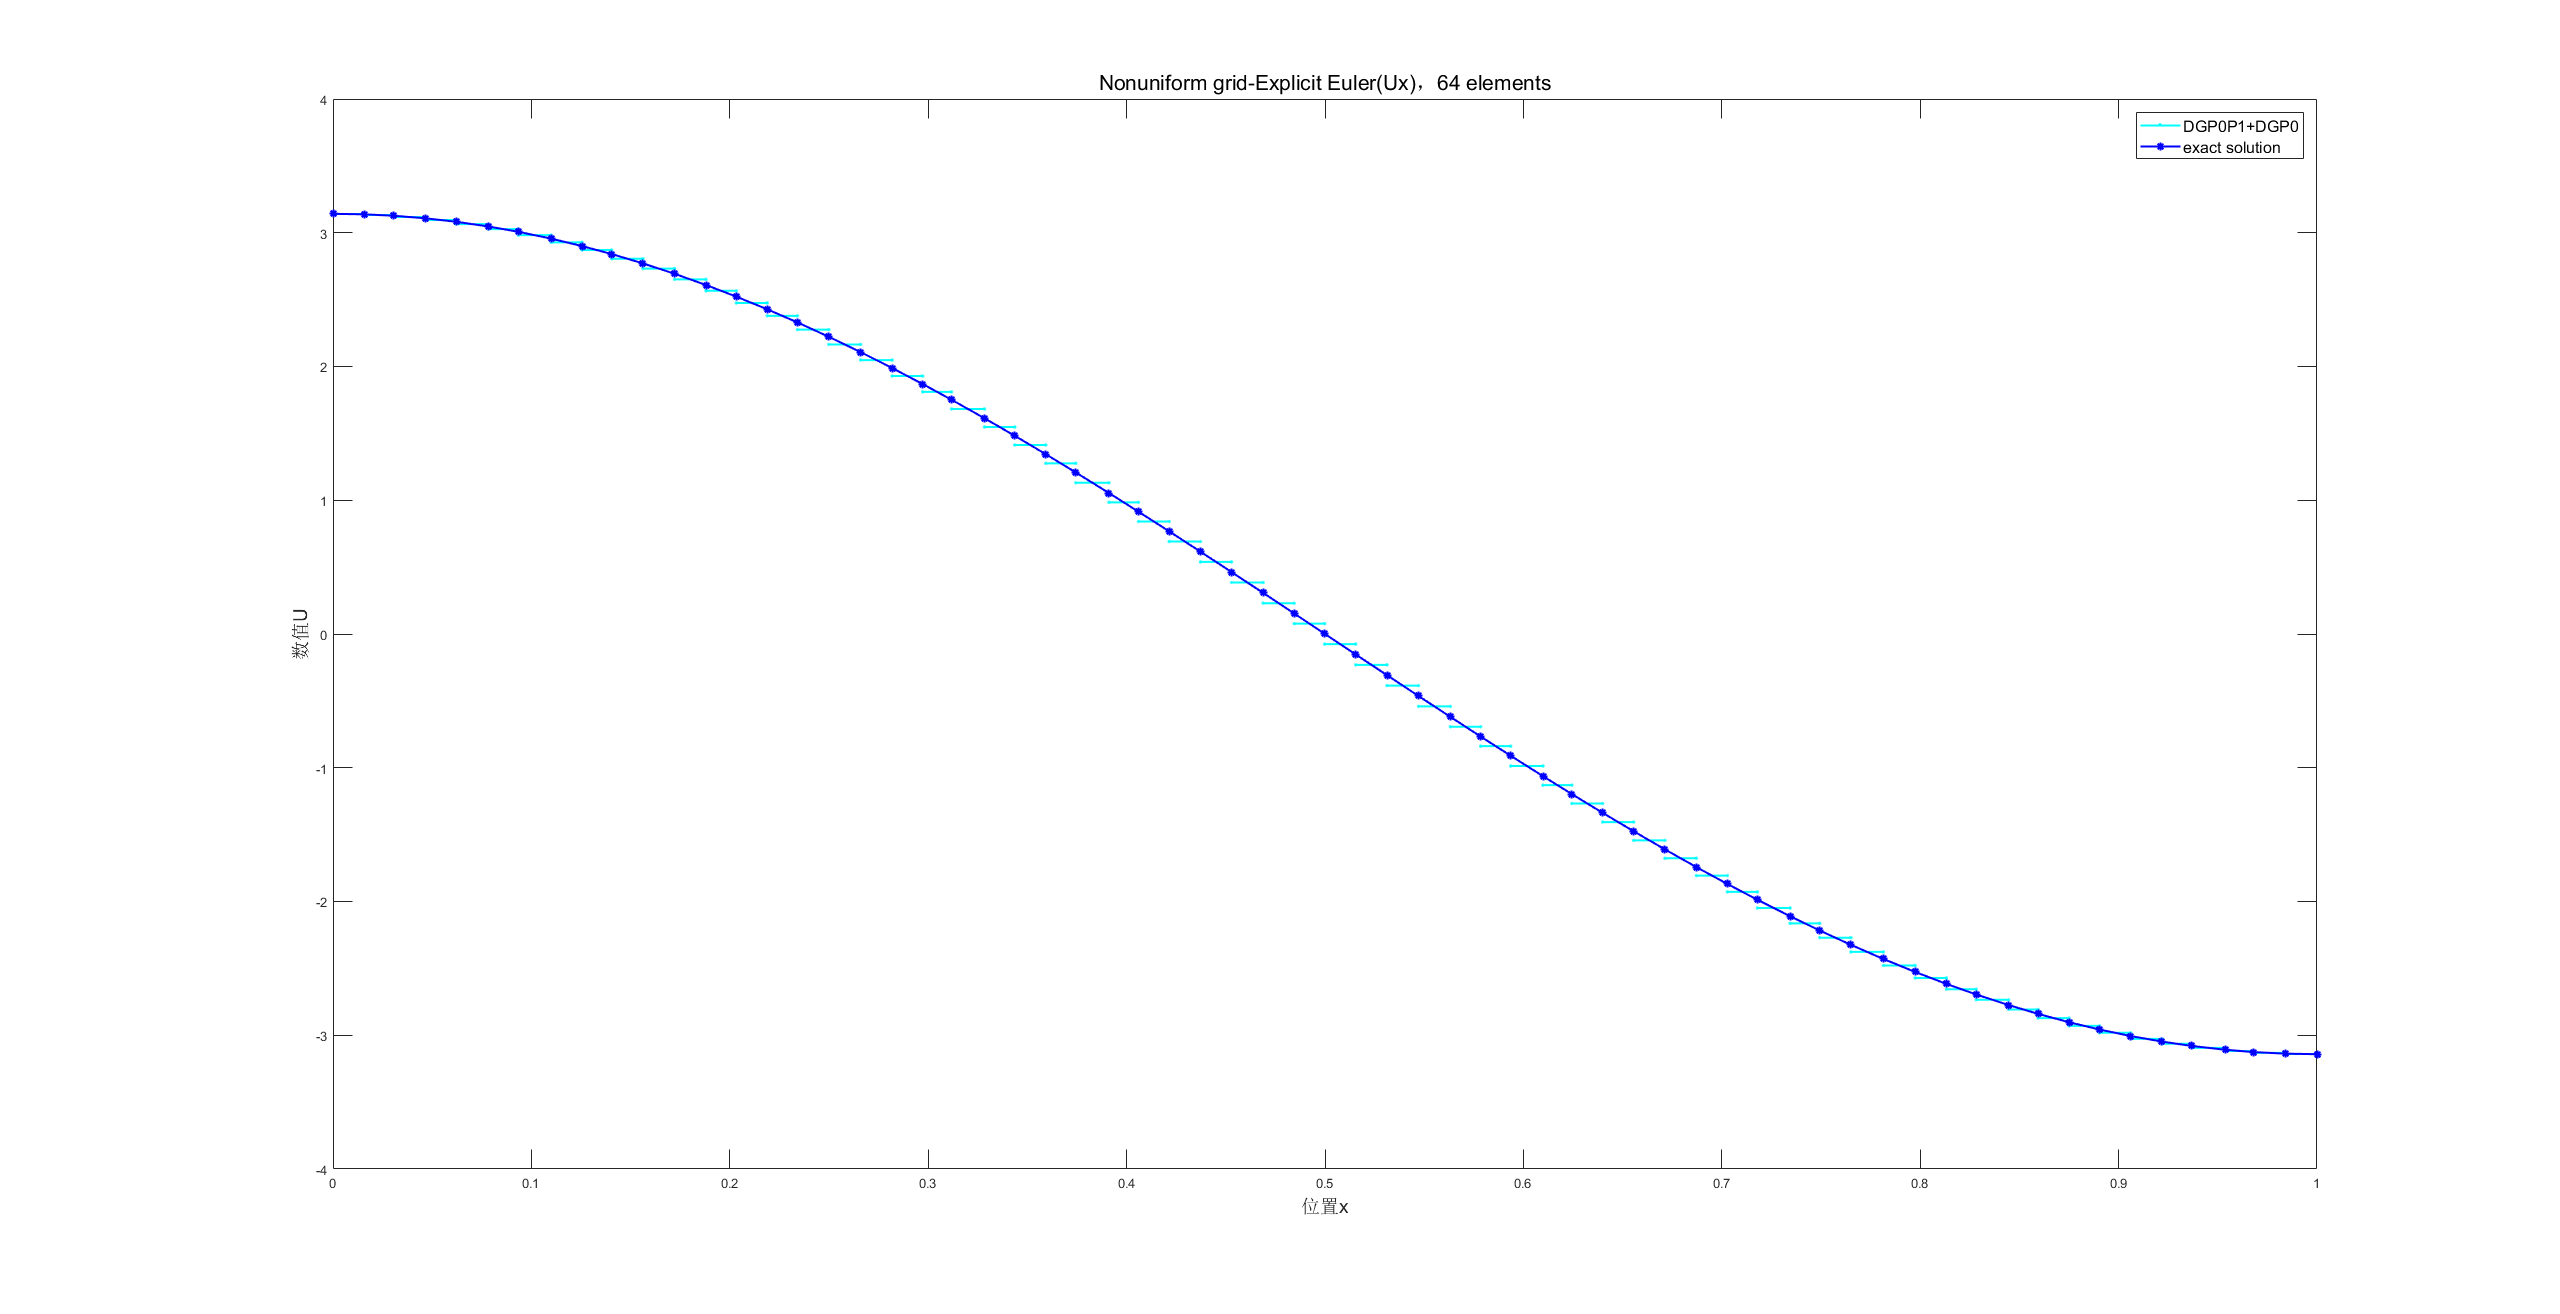
\includegraphics[width=3in]{ununiform grid obviouseuler/Ux64.png} }
	\caption{Nonuniform grid Explicit euler Ux}
\end{figure}\leavevmode\\

\begin{figure}[!h]
	\centering
	\subfloat[U]{
		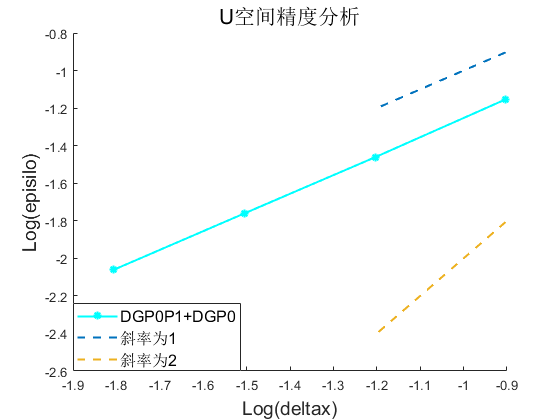
\includegraphics[width=3in]{ununiform grid obviouseuler/U空间精度.png} 
	}
	\hfill
	\subfloat[Ux]{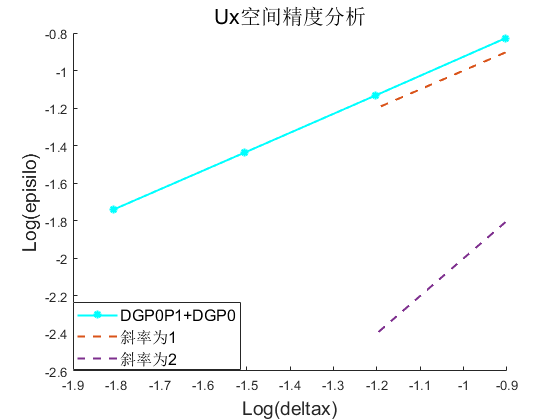
\includegraphics[width=3in]{ununiform grid obviouseuler/Ux空间精度.png} }
	\caption{空间精度}
\end{figure}\leavevmode\\

\clearpage
B)\textbf{Nonuniform grid TVDRK3}\\
\begin{figure}[!h]
	\centering
	\subfloat[8 elements]{
		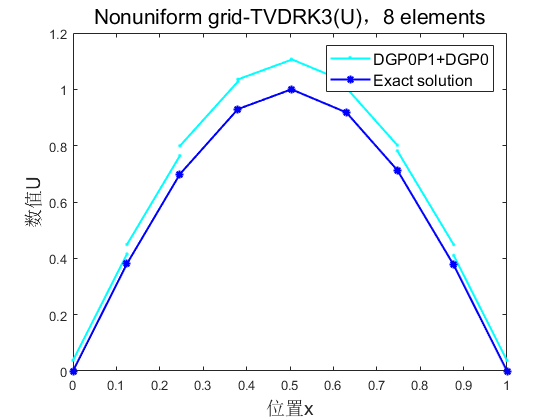
\includegraphics[width=3in]{Ununiform grid TVDRK3/U8.png} 
	}
	\hfill
	\subfloat[64 elements]{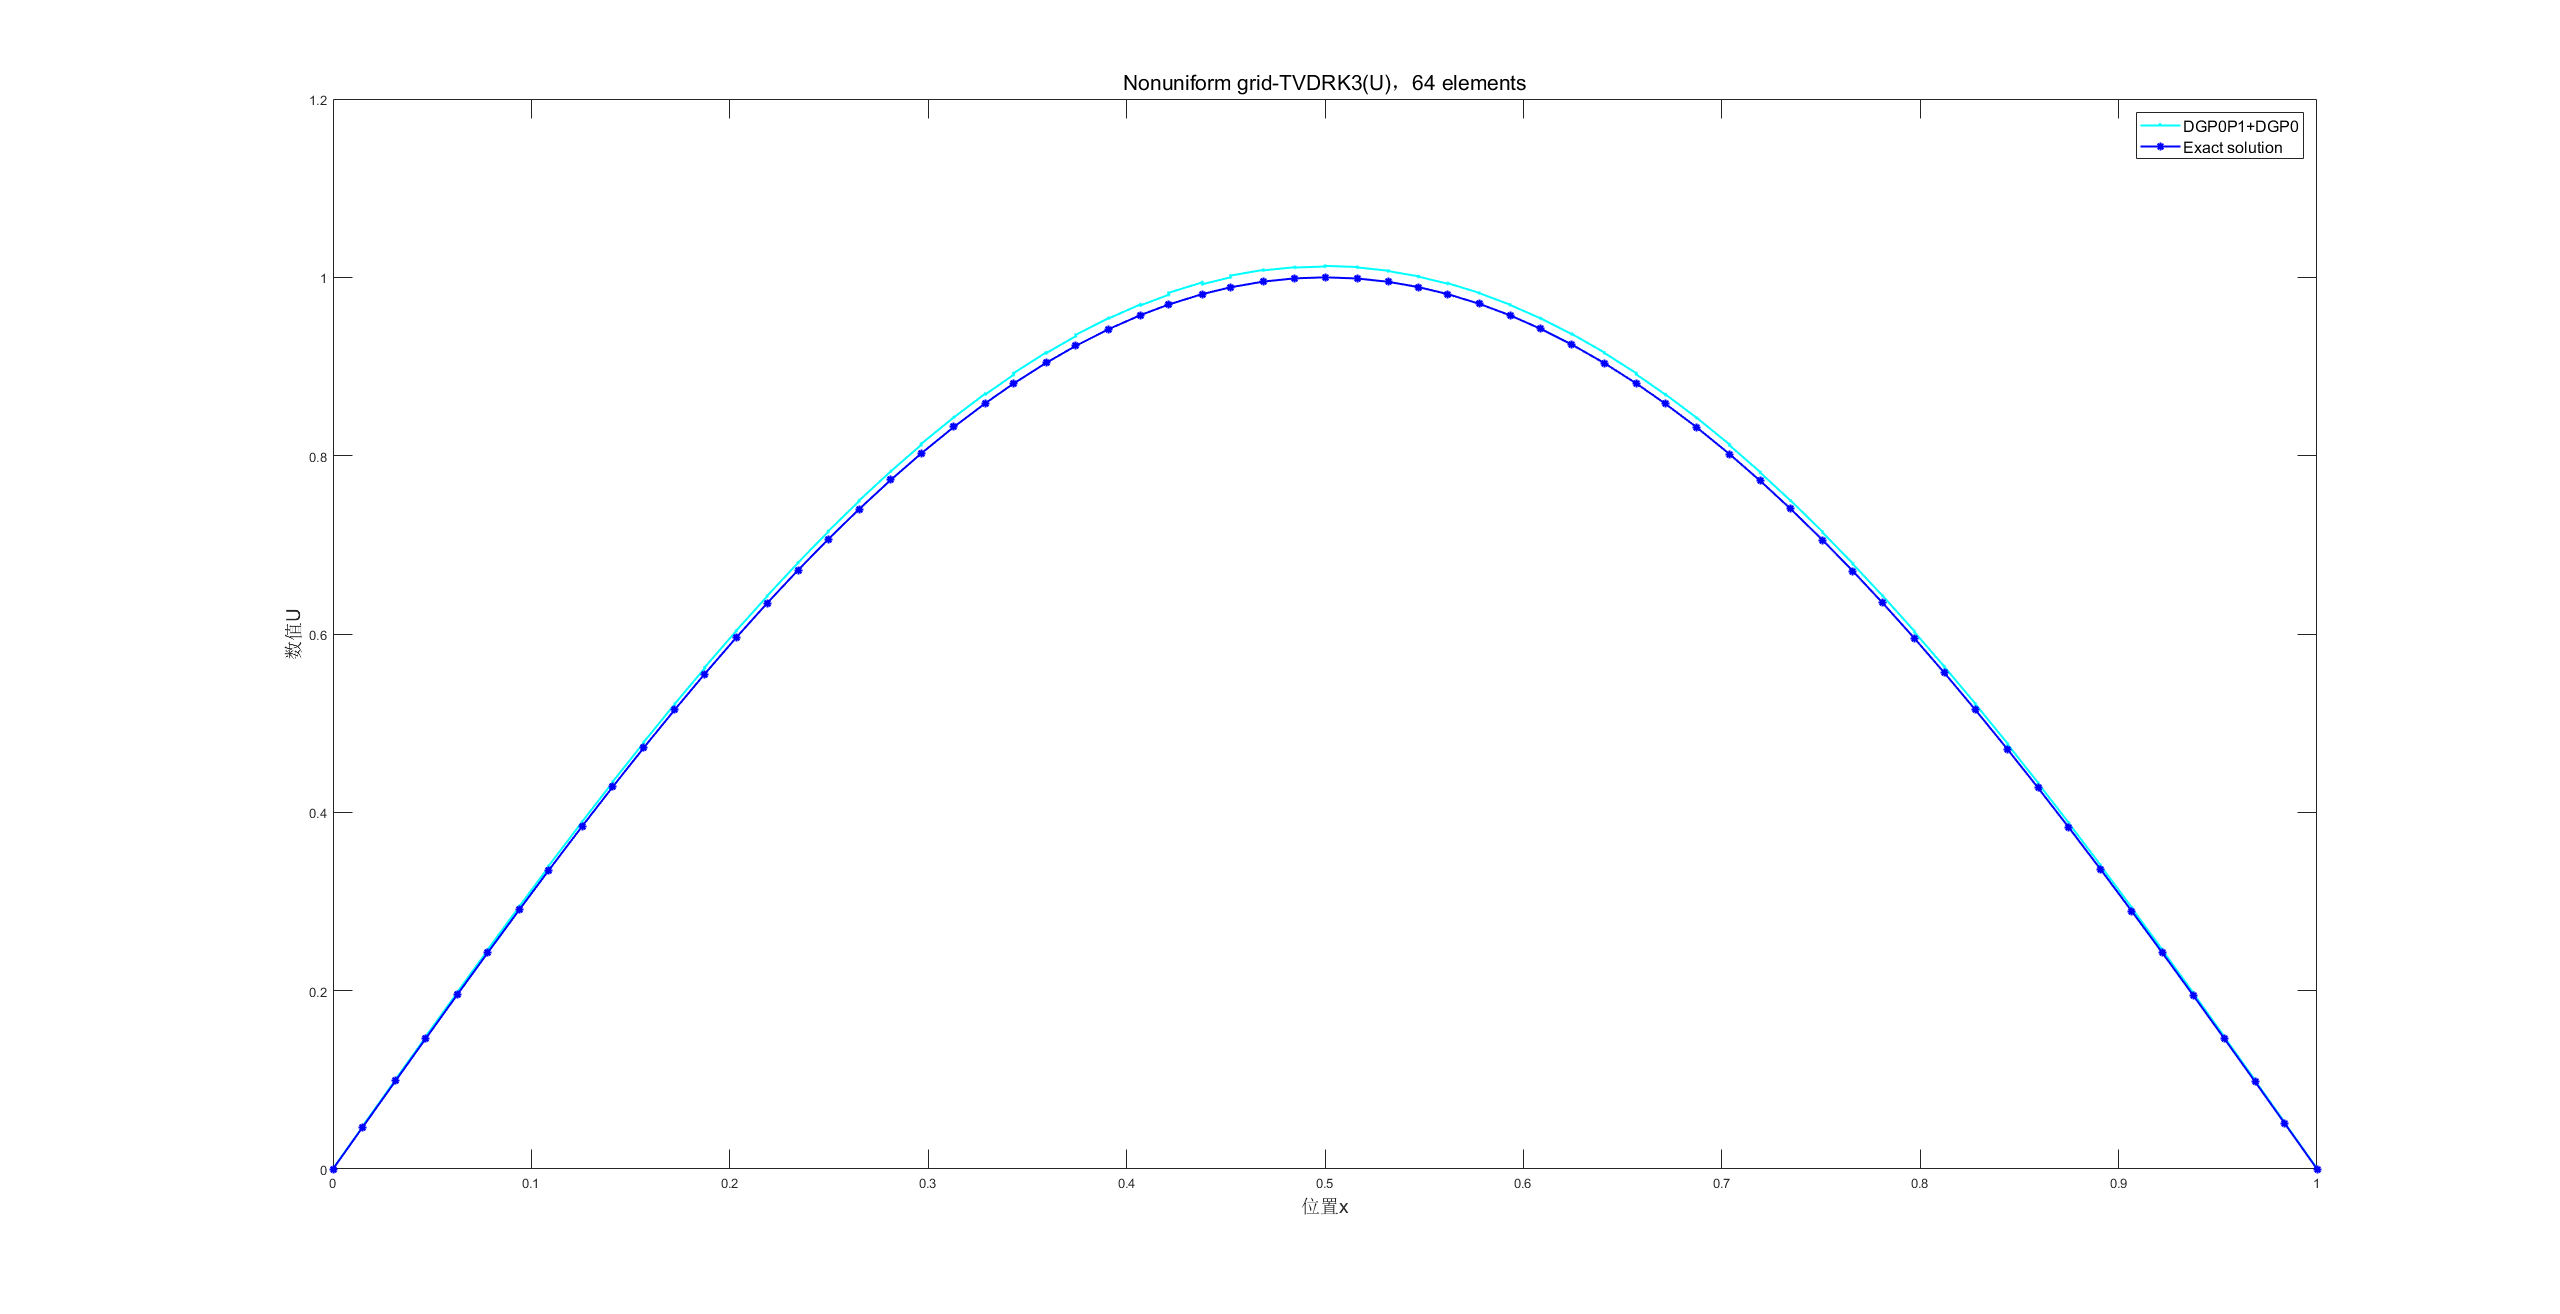
\includegraphics[width=3in]{Ununiform grid TVDRK3/U64.png} }
	\caption{Nonuniform grid TVDRK3 U}
\end{figure}\\


\begin{figure}[!h]
	\centering
	\subfloat[8 elements]{
		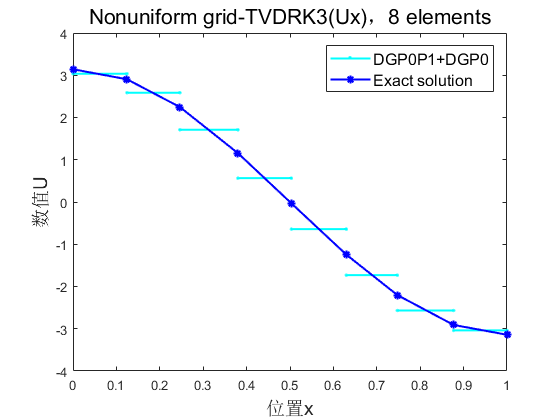
\includegraphics[width=3in]{Ununiform grid TVDRK3/Ux8.png} 
	}
	\hfill
	\subfloat[64 elements]{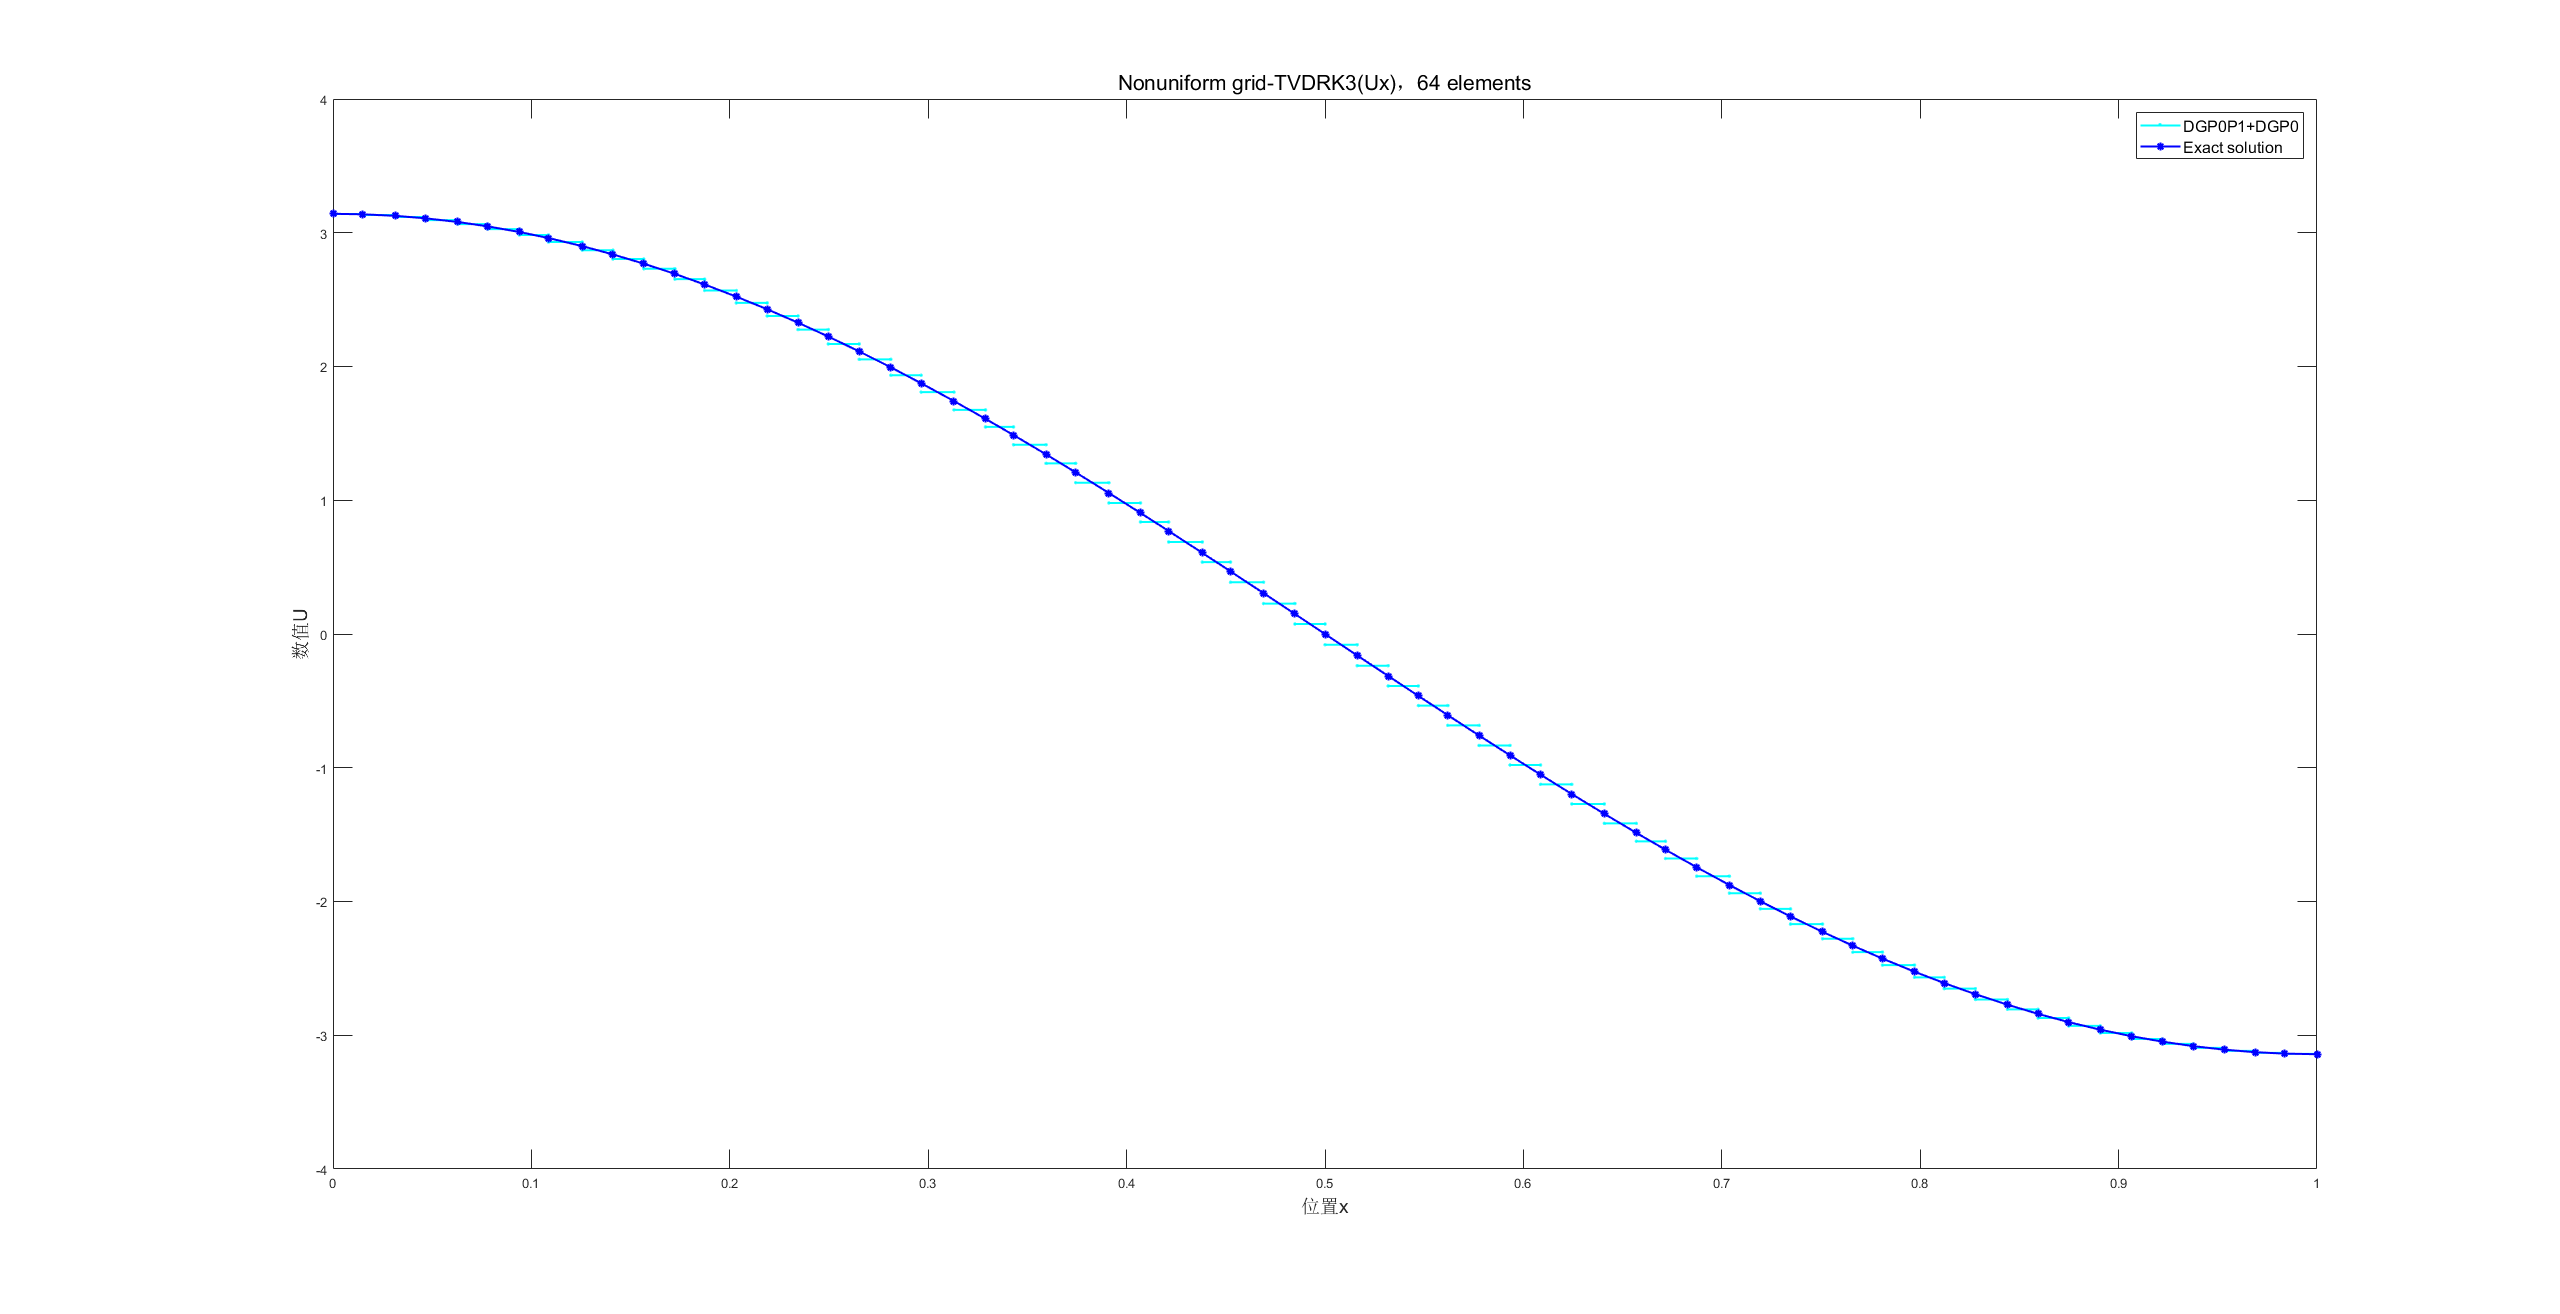
\includegraphics[width=3in]{Ununiform grid TVDRK3/Ux64.png} }
	\caption{Nonuniform grid TVDRK3 Ux}
\end{figure}\leavevmode\\

\begin{figure}[!h]
	\centering
	\subfloat[U]{
		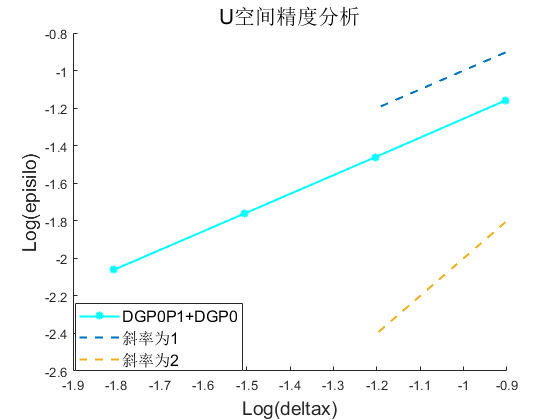
\includegraphics[width=3in]{Ununiform grid TVDRK3/U空间精度.png} 
	}
	\hfill
	\subfloat[Ux]{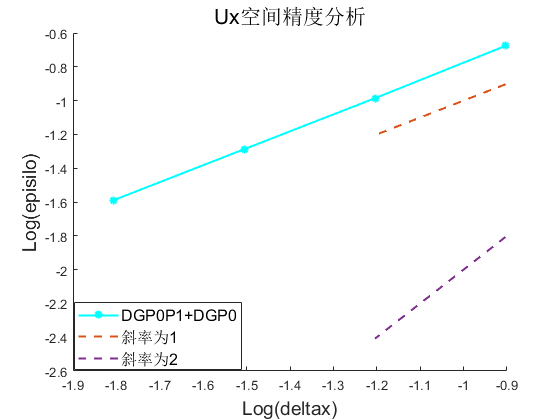
\includegraphics[width=3in]{Ununiform grid TVDRK3/Ux空间精度.png} }
	\caption{空间精度}
\end{figure}\leavevmode\\

\clearpage
C)\textbf{Nonuniform grid BDF1}\\
\begin{figure}[!h]
	\centering
	\subfloat[8 elements]{
		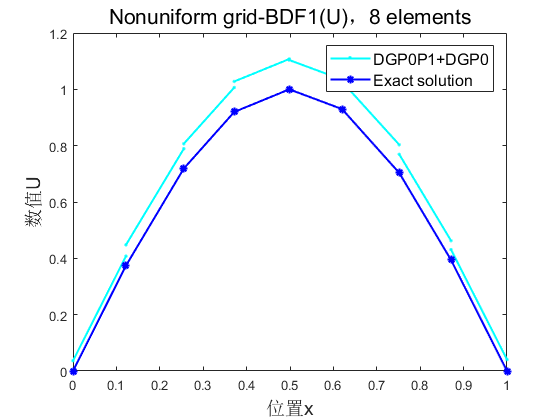
\includegraphics[width=3in]{Ununiform grid BDF1/U8.png} 
	}
	\hfill
	\subfloat[64 elements]{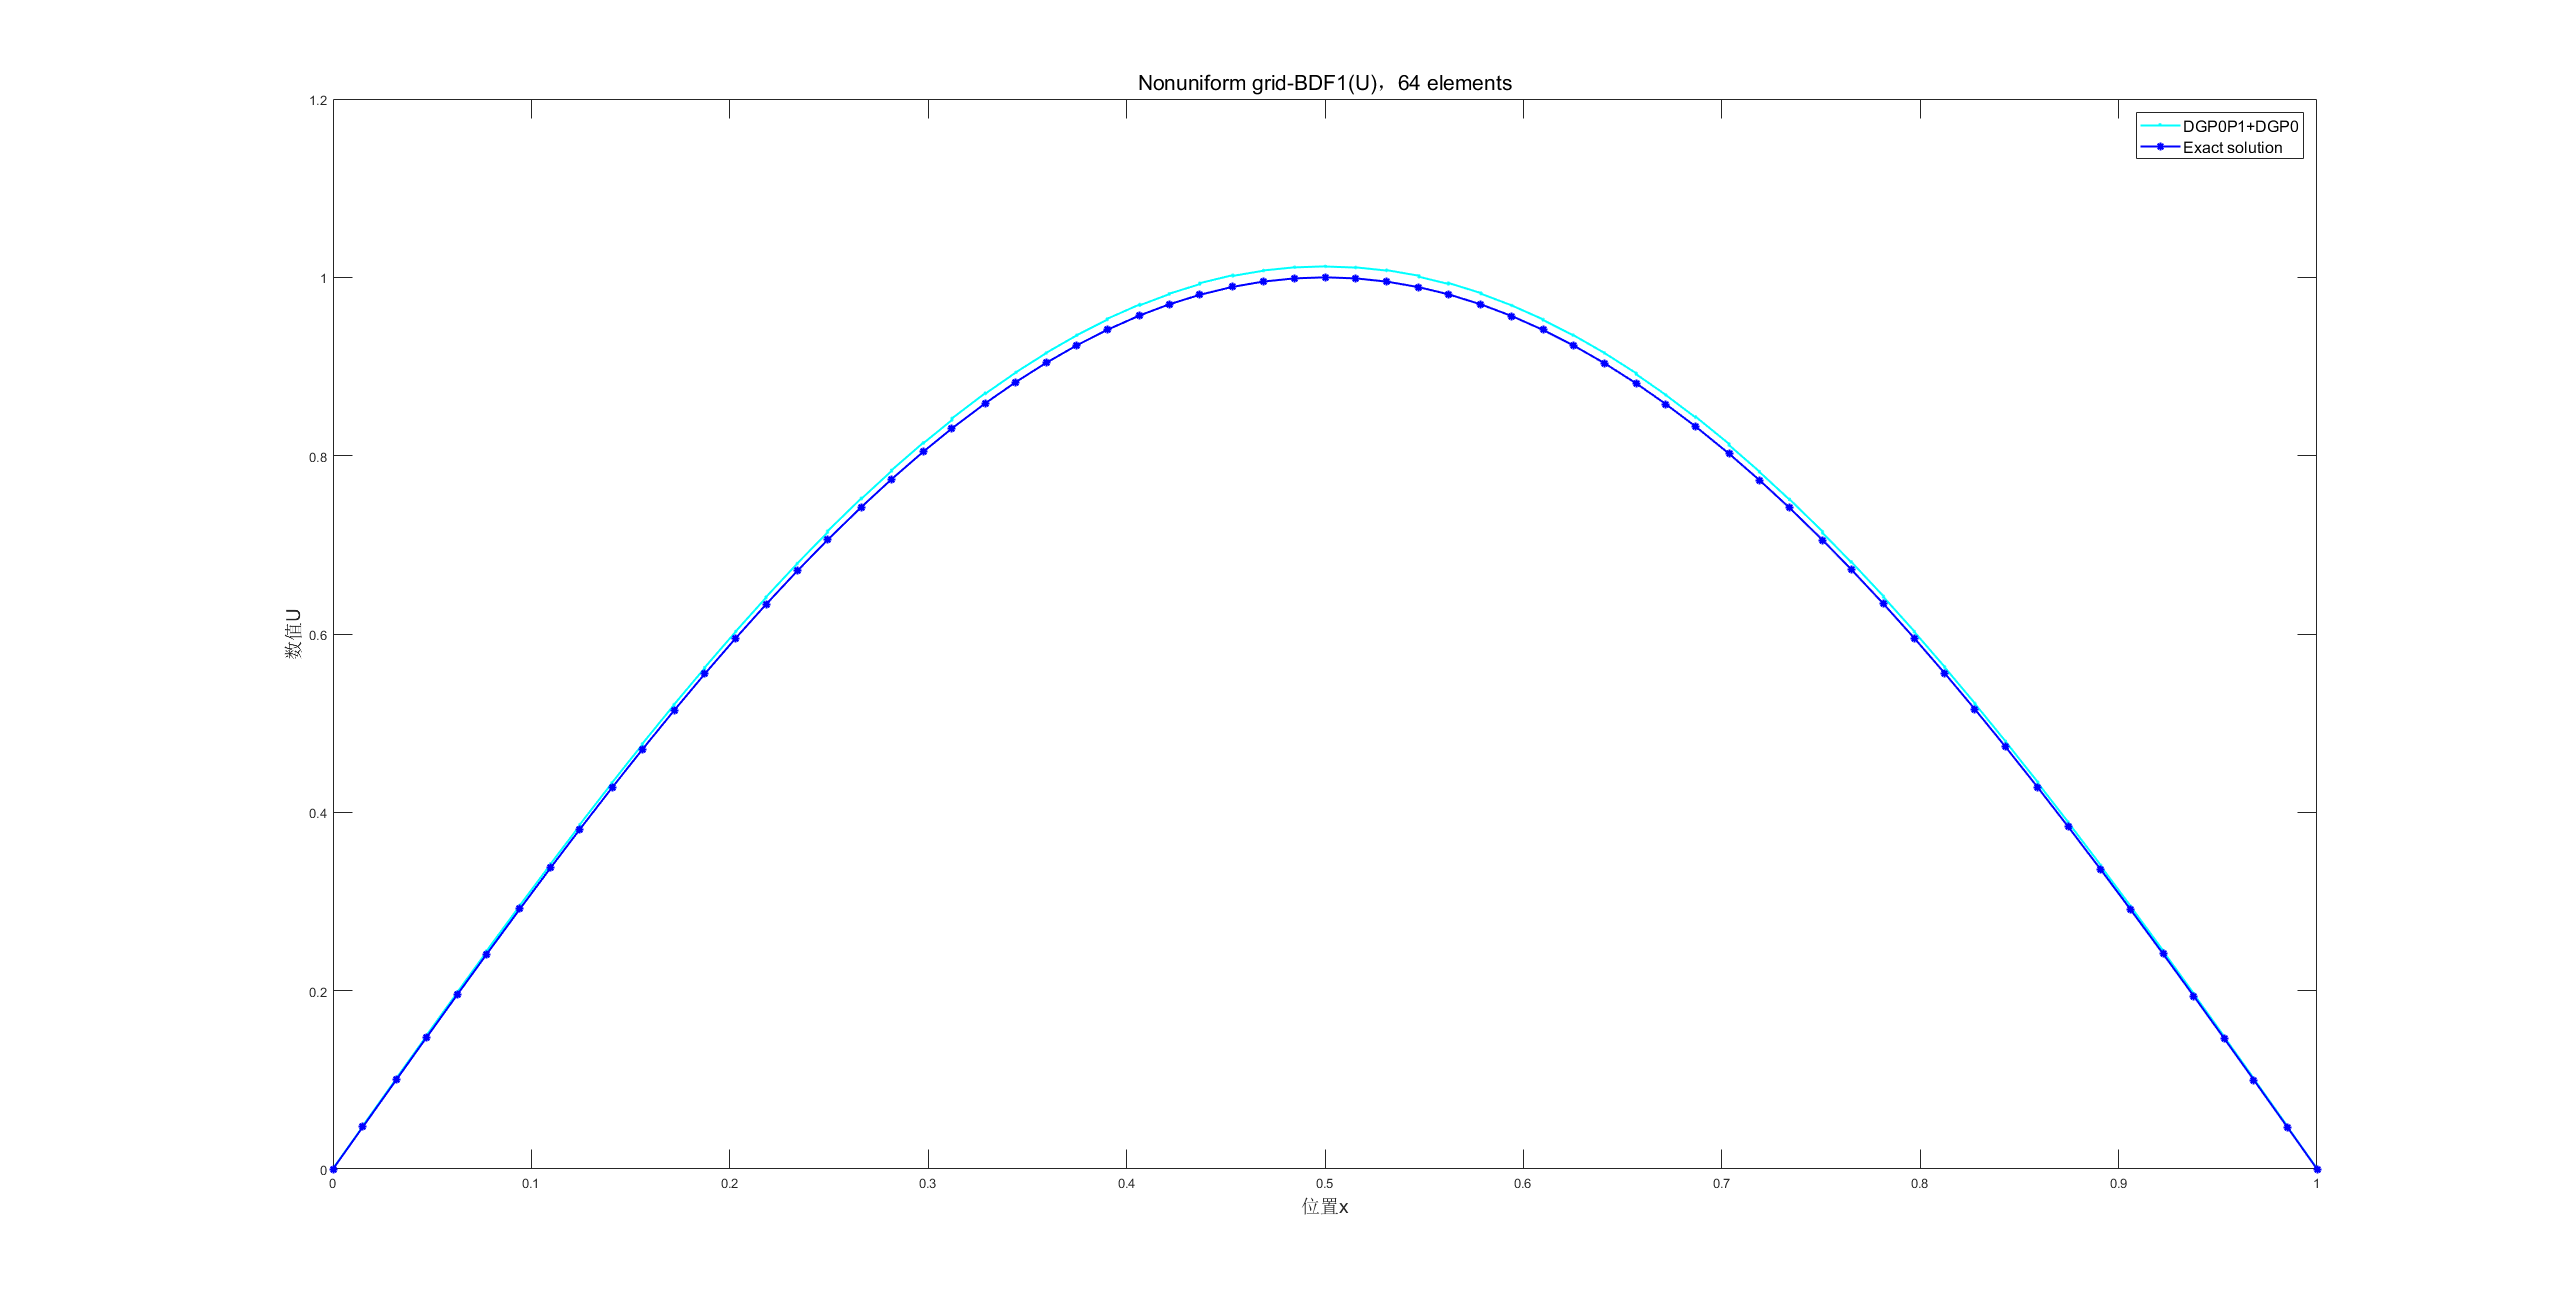
\includegraphics[width=3in]{Ununiform grid BDF1/U64.png} }
	\caption{Nonuniform grid BDF1 U}
\end{figure}\\


\begin{figure}[!h]
	\centering
	\subfloat[8 elements]{
		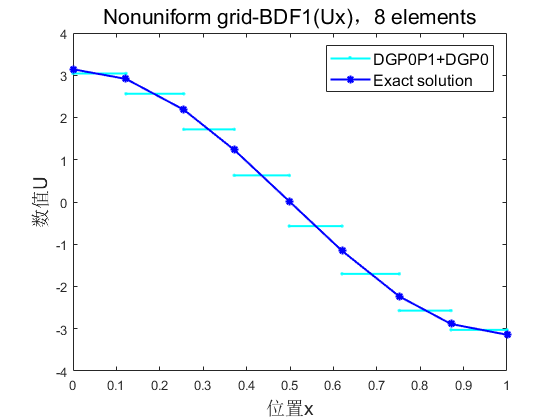
\includegraphics[width=3in]{Ununiform grid BDF1/Ux8.png} 
	}
	\hfill
	\subfloat[64 elements]{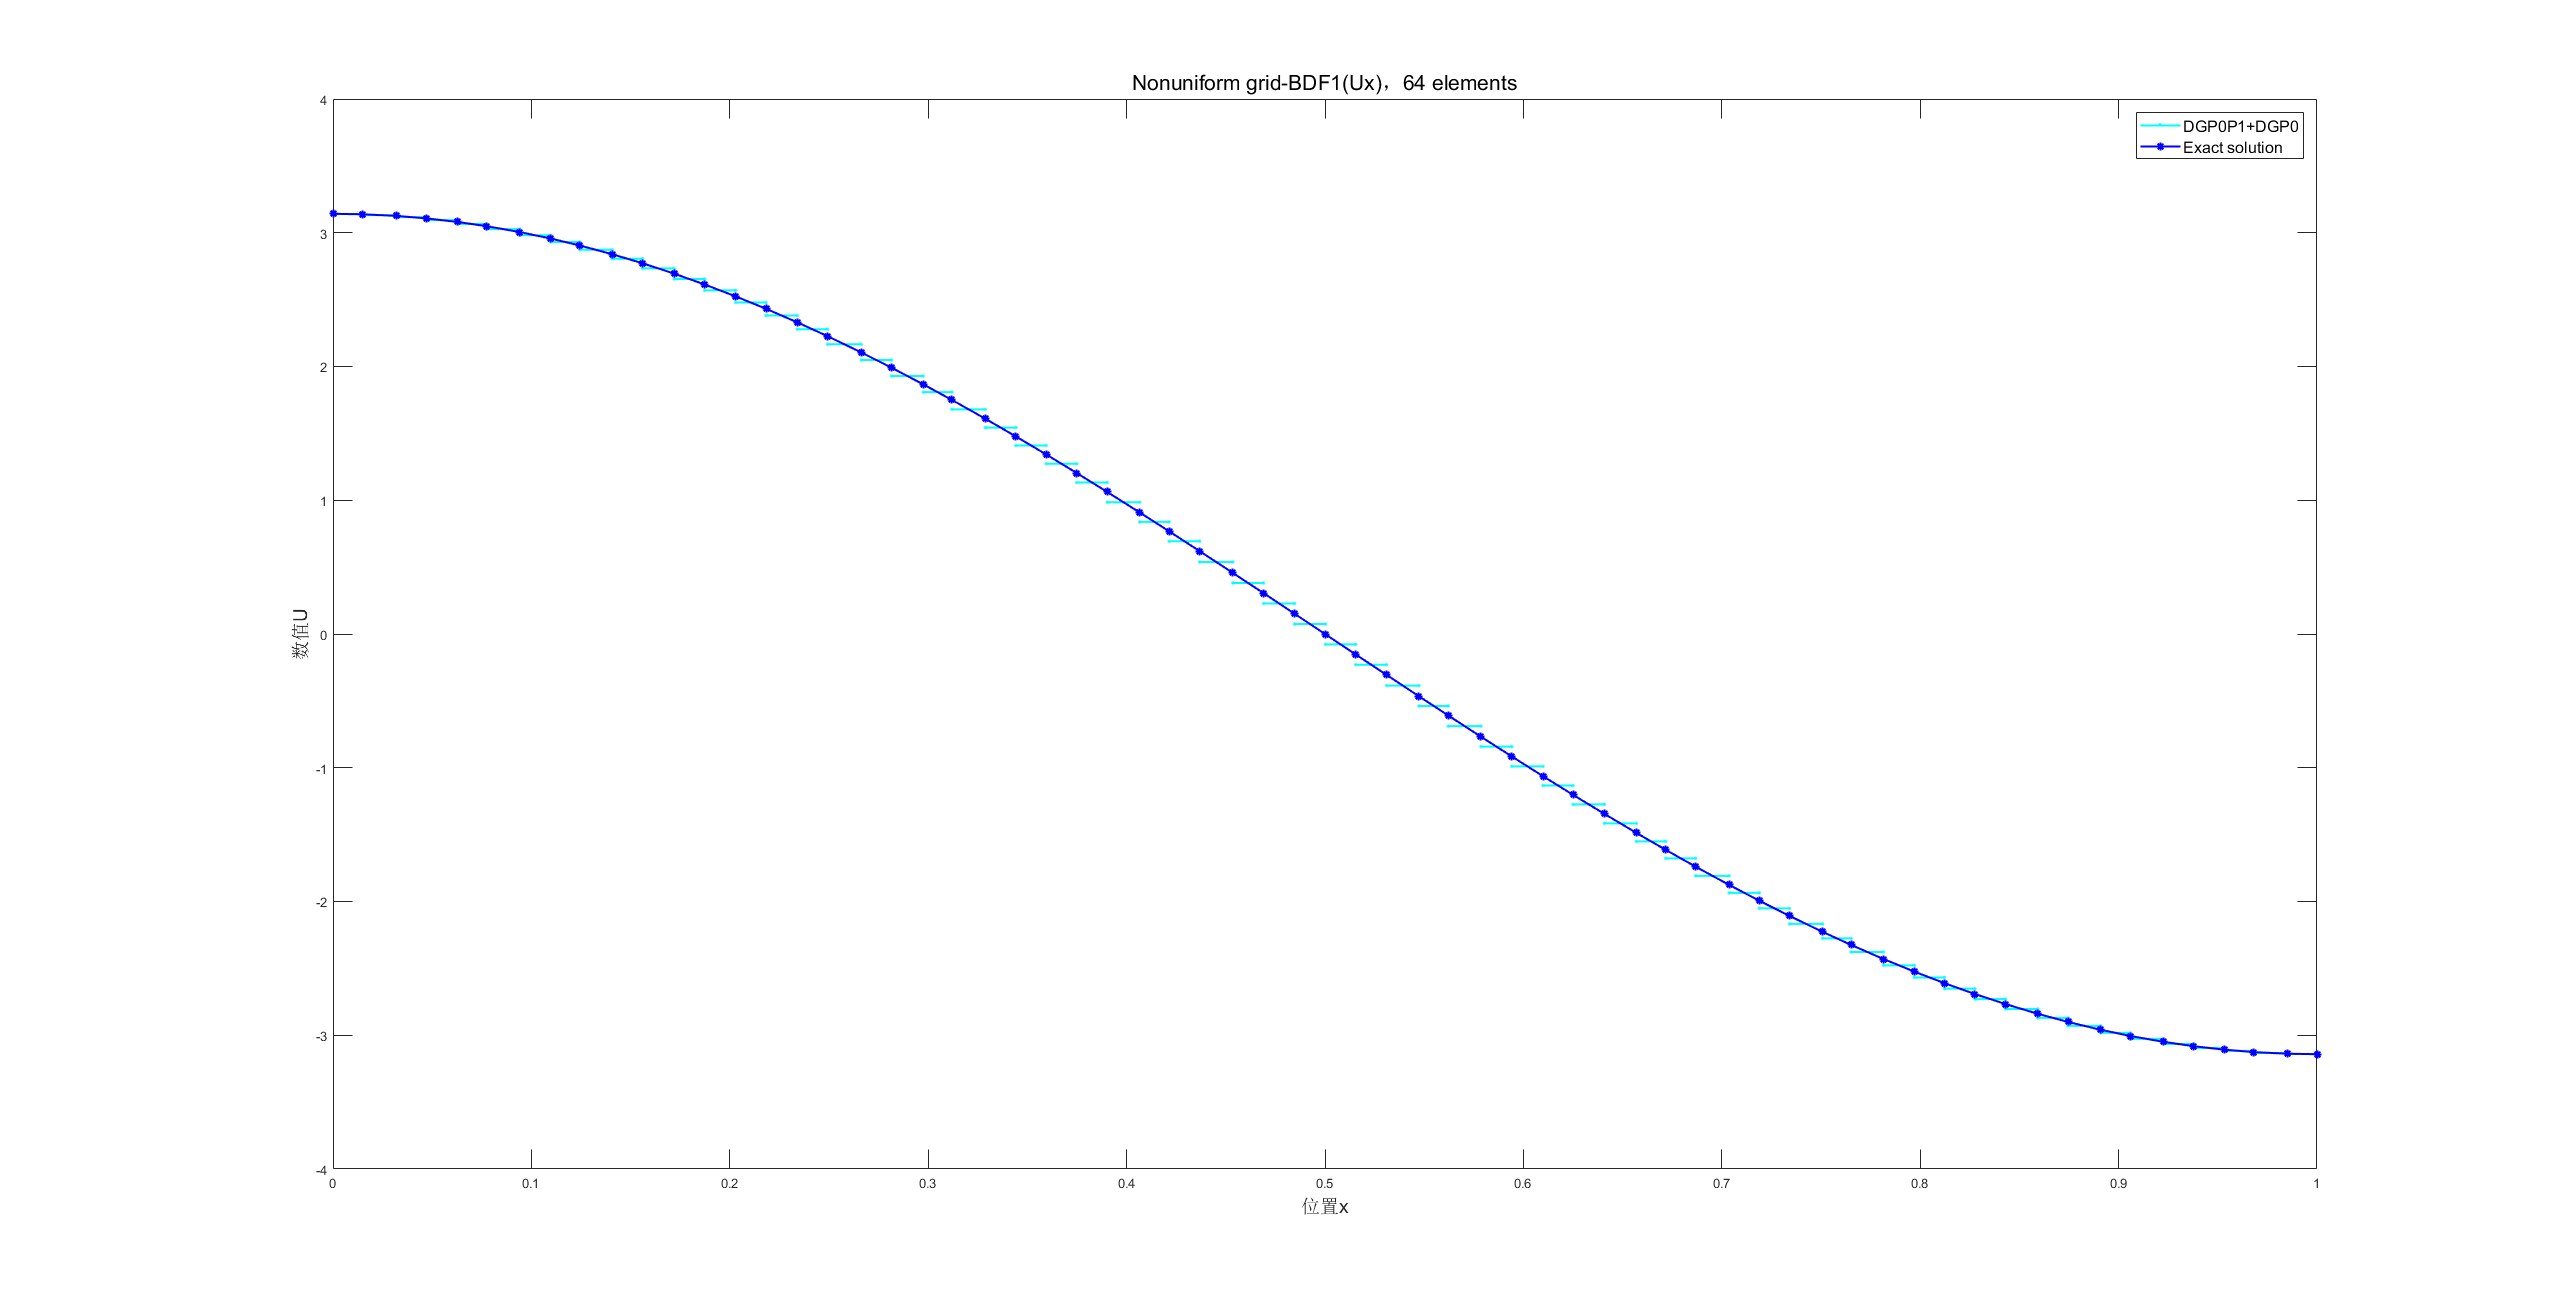
\includegraphics[width=3in]{Ununiform grid BDF1/Ux64.png} }
	\caption{Nonuniform grid BDF1 Ux}
\end{figure}\leavevmode\\

\begin{figure}[!h]
	\centering
	\subfloat[U]{
		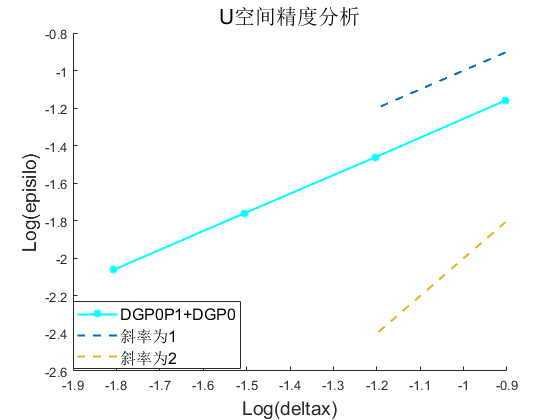
\includegraphics[width=3in]{Ununiform grid BDF1/U空间精度分析.png} 
	}
	\hfill
	\subfloat[Ux]{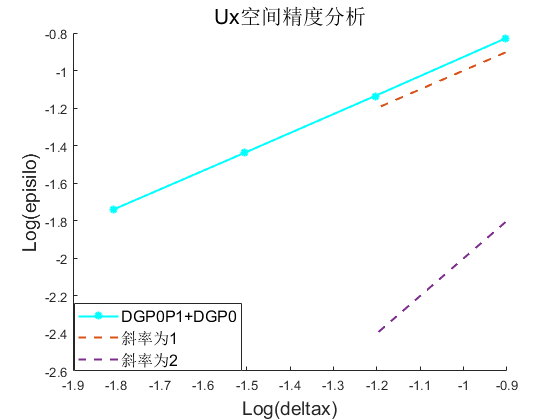
\includegraphics[width=3in]{Ununiform grid BDF1/Ux空间精度分析.png} }
	\caption{空间精度}
\end{figure}\leavevmode\\
\clearpage
\textbf{解:}\\
\indent 2.以下对$f\left(x\right),g\left(x\right)$进行均匀网格与非均匀网格下的P1P2 Green-Gauss Reconstruction,并给出非均匀网格下的重构精度图(仍然采取均匀网格的$\Delta x$).\\
A)\textbf{Uniform grid}\\
\begin{figure}[!h]
	\centering
	\subfloat[f 重构]{
		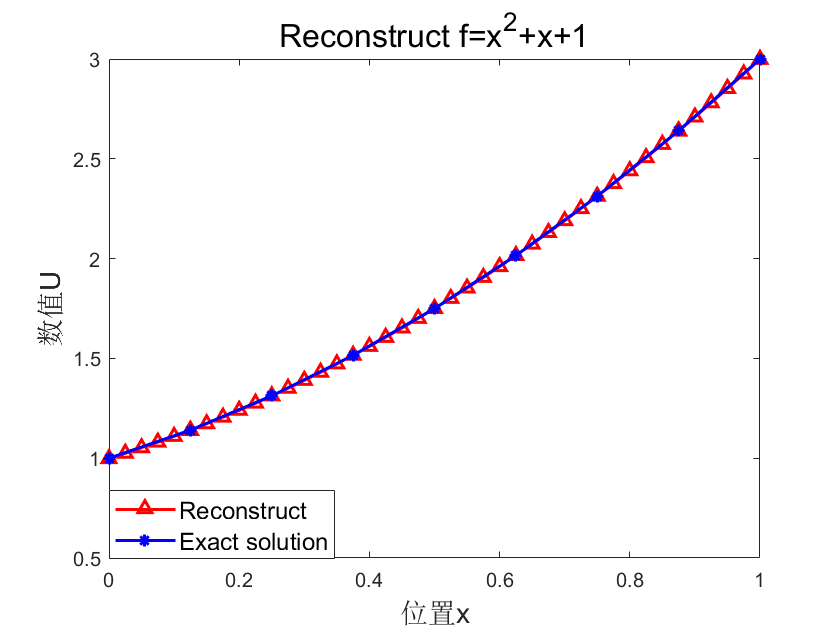
\includegraphics[width=3in]{Green gauss/f重构.png} 
	}
	\hfill
	\subfloat[g 重构]{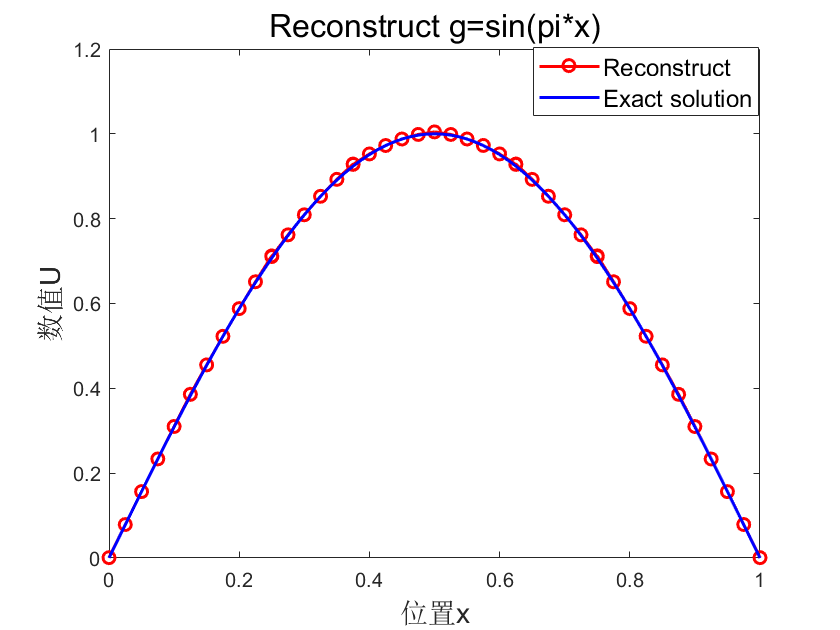
\includegraphics[width=3in]{Green gauss/g重构.png} }
	\caption{Uniform grid Green gauss Reconstruction}
\end{figure}\leavevmode \\

\noindent B)\textbf{Nonuniform grid}\\
\begin{figure}[!h]
	\centering
	\subfloat[f 重构]{
		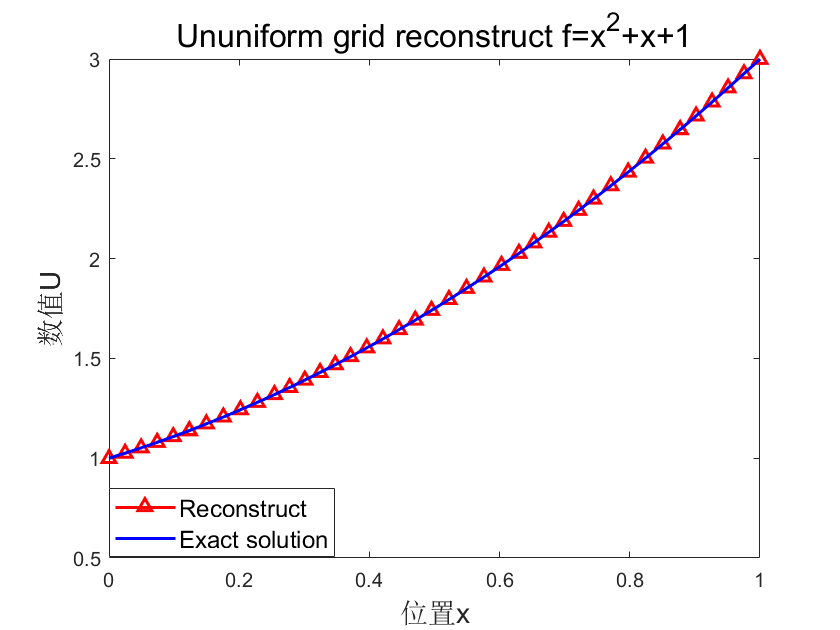
\includegraphics[width=3in]{Green gauss/f重构Uniformgrid.png} 
	}
	\hfill
	\subfloat[g 重构]{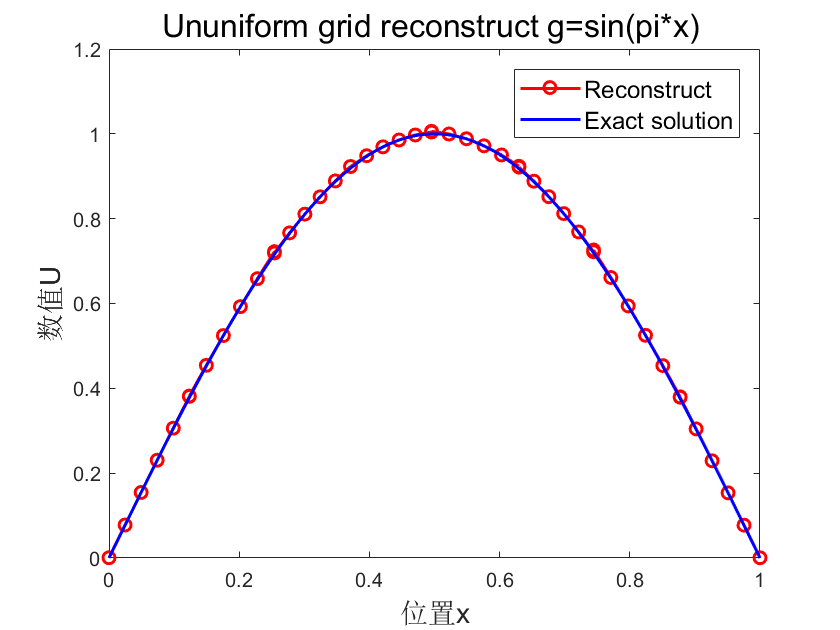
\includegraphics[width=3in]{Green gauss/g重构Uniformgrid.png} }
	\caption{Nonuniform grid Green gauss Reconstruction}
\end{figure}\leavevmode \\


\begin{figure}[!h]
	\centering
	\subfloat[f 重构]{
		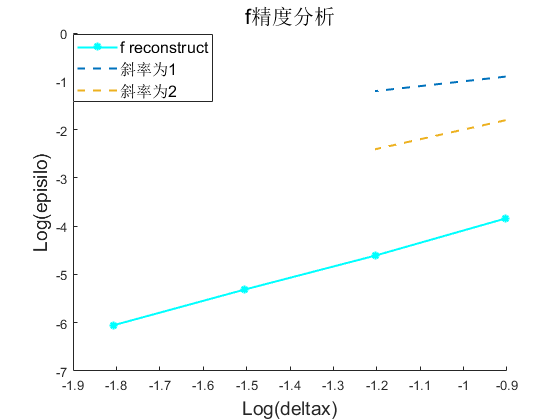
\includegraphics[width=3in]{Green gauss/f精度分析.png} 
	}
	\hfill
	\subfloat[g 重构]{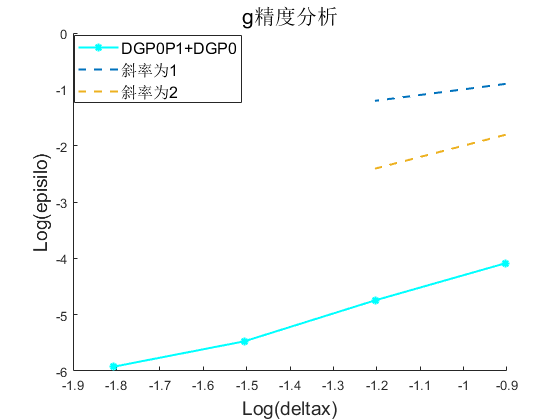
\includegraphics[width=3in]{Green gauss/g精度分析.png} }
	\caption{精度分析}
\end{figure}\leavevmode \\

\clearpage
\section{附录(代码,仅展示部分)}
\noindent \textbf{Nonuniform grid BDF1}
\lstset{language=Matlab}%代码语言使用的是matlab
\lstset{breaklines}%自动将长的代码行换行排版
\lstset{extendedchars=false}%解决代码跨页时,章节标题,页眉等汉字不显示的问题
\begin{lstlisting}
clc
clear all
close all
% Pre-processing
Unit=64;CFL=0.01;endtau=2;endx=1;deltax=1/Unit;numberx=endx/deltax+1;
%记录内点位置
Uexasolution=zeros(2,numberx);
UDGP0P1plusDGP0=zeros(2,numberx-1);
Unumsolution1=zeros(1,2);
Unumsolution2=zeros(2,numberx-1);
Acc=zeros(3,4);a1=[1/8,1/16,1/32,1/64];a2=[1/8,1/16];
% solve the question
%solve the numsolution
[UDGP0P1plusDGP0,Grid,endtau01plus0]=BDF1subDGP0P1plusDGP0(Unit,CFL,endtau);%acquire u and ux
	
%solve the exasolution
x=0;
for k=1:numberx
x=Grid(1,k);
Uexasolution(1,k)=sin(pi*x);
Uexasolution(2,k)=pi*cos(pi*x);
end
% post-processing
%plot the u
%plot the DGP0P1plusDGP0
figure
Unumsolution1(1,1)=UDGP0P1plusDGP0(1,1)-UDGP0P1plusDGP0(2,1)*(Grid(2)-Grid(1))/2;Unumsolution1(1,2)=UDGP0P1plusDGP0(1,1)+UDGP0P1plusDGP0(2,1)*(Grid(2)-Grid(1))/2;
plot([Grid(1,1),Grid(1,2)],Unumsolution1,'-c.','linewidth',1.5);hold on
H1=plot([Grid(1,1),Grid(1,2)],Unumsolution1,'-c.','linewidth',1.5);hold on
for i=2:numberx-1
Unumsolution1(1,1)=UDGP0P1plusDGP0(1,i)-UDGP0P1plusDGP0(2,i)*(Grid(i+1)-Grid(i))/2;Unumsolution1(1,2)=UDGP0P1plusDGP0(1,i)+UDGP0P1plusDGP0(2,i)*(Grid(i+1)-Grid(i))/2;
plot([Grid(1,i),Grid(1,i+1)],Unumsolution1,'-c.','linewidth',1.5)
end
	
%plot the exact
y=Grid;
plot(y,Uexasolution(1,:),'-b*','linewidth',1.5)
H2=plot(y,Uexasolution(1,:),'-b*','linewidth',1.5);hold on
lgd=legend([H1,H2],'DGP0P1+DGP0','Exact solution');
lgd.FontSize=12;
xlabel('位置x','fontsize',14)
ylabel('数值U','fontsize',14)
title('Ununiform grid-BDF1(U),64 element','fontsize',16)
hold off
	
	
%plot the ux
%DGP0P1plusDGP0
figure
Unumsolution1(1,1)=UDGP0P1plusDGP0(2,1);Unumsolution1(1,2)=UDGP0P1plusDGP0(2,1);
plot([Grid(1,1),Grid(1,2)],Unumsolution1,'-c.','linewidth',1.5);hold on
H1=plot([Grid(1,1),Grid(1,2)],Unumsolution1,'-c.','linewidth',1.5);hold on
for i=2:numberx-1
Unumsolution1(1,1)=UDGP0P1plusDGP0(2,i);Unumsolution1(1,2)=UDGP0P1plusDGP0(2,i);
plot([Grid(1,i),Grid(1,i+1)],Unumsolution1,'-c.','linewidth',1.5)
end
	
%exact
y=Grid;
plot(y,Uexasolution(2,:),'-b*','linewidth',1.5)
H2=plot(y,Uexasolution(2,:),'-b*','linewidth',1.5);hold on
lgd=legend([H1,H2],'DGP0P1+DGP0','Exact solution');
lgd.FontSize=12;
xlabel('位置x','fontsize',14)
ylabel('数值U','fontsize',14)
title('Ununiform grid-BDF1(Ux),64 element','fontsize',16)
hold off
	
%determine the accuracy of space U
[U,G,~]=BDF1subDGP0P1plusDGP0(8,CFL,endtau);
Acc(1,1)=AccuracyU(8,U,G);
[U,G,~]=BDF1subDGP0P1plusDGP0(16,CFL,endtau);
Acc(1,2)=AccuracyU(16,U,G);
[U,G,~]=BDF1subDGP0P1plusDGP0(32,CFL,endtau);
Acc(1,3)=AccuracyU(32,U,G);
[U,G,~]=BDF1subDGP0P1plusDGP0(64,CFL,endtau);
Acc(1,4)=AccuracyU(64,U,G);
	
figure
hold on
plot(log10(a1),log10(Acc(1,:)),'-c*','linewidth',1.5)
H1=plot(log10(a1),log10(Acc(1,:)),'-c*','linewidth',1.5);
	
H2=plot(log10(a2),1*log10(a2),'--','linewidth',1.5);
plot(log10(a2),2*log10(a2),'--','linewidth',1.5)
H3=plot(log10(a2),2*log10(a2),'--','linewidth',1.5);
lgd=legend([H1,H2,H3],'DGP0P1+DGP0','斜率为1','斜率为2');
lgd.FontSize=12;
xlabel('Log(deltax)','fontsize',14)
ylabel('Log(episilo)','fontsize',14)
title('U空间精度分析','fontsize',16)
	
%determine the accuracy of space Ux
%DGP0P1
[U,G,~]=BDF1subDGP0P1plusDGP0(8,CFL,endtau);
Acc(1,1)=AccuracyUx(8,U,G);
[U,G,~]=BDF1subDGP0P1plusDGP0(16,CFL,endtau);
Acc(1,2)=AccuracyUx(16,U,G);
[U,G,~]=BDF1subDGP0P1plusDGP0(32,CFL,endtau);
Acc(1,3)=AccuracyUx(32,U,G);
[U,G,~]=BDF1subDGP0P1plusDGP0(64,CFL,endtau);
Acc(1,4)=AccuracyUx(64,U,G);
	
figure
hold on
plot(log10(a1),log10(Acc(1,:)),'-c*','linewidth',1.5)
H1=plot(log10(a1),log10(Acc(1,:)),'-c*','linewidth',1.5);
	
plot(log10(a2),1*log10(a2),'--','linewidth',1.5)
H2=plot(log10(a2),1*log10(a2),'--','linewidth',1.5);
plot(log10(a2),2*log10(a2),'--','linewidth',1.5)
H3=plot(log10(a2),2*log10(a2),'--','linewidth',1.5);
lgd=legend([H1,H2,H3],'DGP0P1+DGP0','斜率为1','斜率为2');
lgd.FontSize=12;
xlabel('Log(deltax)','fontsize',14)
ylabel('Log(episilo)','fontsize',14)
title('Ux空间精度分析','fontsize',16)
	
\end{lstlisting}

\noindent \textbf{BDF1subDGP0P1plusDGP0}
\begin{lstlisting}
function [Unumsolution,Grid,N]=subDGP0P1plusDGP0(Unit,CFL,endtau)
endx=1;deltax=endx/Unit;tol=10^(-10);
nu=1;Lr=1/(2*pi);Tr=Lr^2/nu;
abslambda=sqrt(nu/Tr);
numberx=Unit+1;
%记录内点位置
Grid=zeros(1,numberx);
for i=2:numberx-1
Grid(1,i)=(i-1)*deltax+(0.1*rand(1)-0.05)*deltax;
end
Grid(1,numberx)=endx;
	
deltatau=zeros(1,numberx-1);
for i=1:numberx-1
deltatau(i)=CFL*(Grid(1,i+1)-Grid(1,i))/abslambda;%伪时间变量
end
	
% Ucurrent=zeros(2,numberx-1);
% Unext=zeros(2,numberx-1);
	
B1=1;
%C=[B1,0;0,B1/deltax];
%Mtau=[deltax,0;0,deltax/12+1/deltax];%此为推导出的U=CV中的C
A=[abslambda,0;0,abslambda];
R=zeros(2*Unit,1);
Rd=zeros(2,numberx-1);
Rb=zeros(2,numberx-1);
Fn=zeros(2,numberx);
	
	
% solve the question
%构建LHS
%Mtau/deltatau
LHS1=zeros(2*Unit,2*Unit);
for k=1:numberx-1
LHS1(2*k-1,2*k-1)=(Grid(k+1)-Grid(k))/deltatau(k);
LHS1(2*k,2*k)=((Grid(k+1)-Grid(k))/12+1/(Grid(k+1)-Grid(k)))/deltatau(k);
end
%Rdomain
for k=1:numberx-1
LHS2(2*k,2*k)=(nu+1/Tr)/(Grid(k+1)-Grid(k));
end
	
%Rboundary
LHS3=zeros(2*Unit,2*Unit);
for iface=2:numberx-1
ieL=iface-1;
ieR=iface;
CL=[B1,1/2;0,B1/(Grid(ieL+1)-Grid(ieL))];
CR=[B1,-1/2;0,B1/(Grid(ieR+1)-Grid(ieR))];
%diag
LHS3(2*ieL-1:2*ieL,2*ieL-1:2*ieL)=LHS3(2*ieL-1:2*ieL,2*ieL-1:2*ieL)+CL'*[abslambda/2,-nu/2;-1/(2*Tr),abslambda/2]*CL;
LHS3(2*ieR-1:2*ieR,2*ieR-1:2*ieR)=LHS3(2*ieR-1:2*ieR,2*ieR-1:2*ieR)-CR'*[-abslambda/2,-nu/2;-1/(2*Tr),-abslambda/2]*CR;
%upper
LHS3(2*ieL-1:2*ieL,2*ieR-1:2*ieR)=LHS3(2*ieL-1:2*ieL,2*ieR-1:2*ieR)+CL'*[-abslambda/2,-nu/2;-1/(2*Tr),-abslambda/2]*CR;
%lower
LHS3(2*ieR-1:2*ieR,2*ieL-1:2*ieL)=LHS3(2*ieR-1:2*ieR,2*ieL-1:2*ieL)-CR'*[abslambda/2,-nu/2;-1/(2*Tr),abslambda/2]*CL;
end
CL=[B1,1/2;0,B1/(Grid(numberx)-Grid(numberx-1))];
CR=[B1,-1/2;0,B1/(Grid(2)-Grid(1))];
LHS3(2*1-1:2*1,2*1-1:2*1)=LHS3(2*1-1:2*1,2*1-1:2*1)-CR'*([abslambda/2,-nu/2;-1/(2*Tr),abslambda/2]*[0,0;0,1/deltax]+[-abslambda/2,-nu/2;-1/(2*Tr),-abslambda/2]*CR);
LHS3(2*(numberx-1)-1:2*(numberx-1),2*(numberx-1)-1:2*(numberx-1))=LHS3(2*(numberx-1)-1:2*(numberx-1),2*(numberx-1)-1:2*(numberx-1))+CL'*([abslambda/2,-nu/2;-1/(2*Tr),abslambda/2]+[-abslambda/2,-nu/2;-1/(2*Tr),-abslambda/2]*[0,0;0,1])*CL;
LHS=LHS1+LHS2+LHS3;
	
%取出我们所需要的D
D=zeros(2*Unit,2*Unit);
for iface=2:numberx
ieL=iface-1;
D(2*ieL-1:2*ieL,2*ieL-1:2*ieL)=LHS(2*ieL-1:2*ieL,2*ieL-1:2*ieL);
end
%为循环所预设的一些量
Ucurrent=zeros(2,numberx-1);
Unext=zeros(2*Unit,1);
%initial  condition set up
	
for k=1:numberx-1
x=Grid(k);
Ucurrent(1,k)=(x+(Grid(k+1)-Grid(k))/2)^2-(x+(Grid(k+1)-Grid(k))/2);
Ucurrent(2,k)=(2*(x+(Grid(k+1)-Grid(k))/2)-1)*(Grid(k+1)-Grid(k));%Ucurrent(2,:)存储的是Ux*deltx
end
	
%Rdomain
for k=1:numberx-1
Rd(1,k)=gauss1(Grid(k),Grid(k+1));
%Rd(1,k)=pi*(cos(pi*x)-cos(pi*(x+deltax)));
%Rd(2,k)=-nu*Ucurrent(2,k)/deltax+(-pi/deltax*(deltax/2*cos(pi*(x+deltax))-(-deltax/2)*cos(pi*x)-1/pi*(sin(pi*(x+deltax))-sin(pi*x))))-Ucurrent(2,k)/(Tr*deltax);
Rd(2,k)=-nu*Ucurrent(2,k)/(Grid(k+1)-Grid(k))-Ucurrent(2,k)/(Tr*(Grid(k+1)-Grid(k)))+gauss2(Grid(k),Grid(k+1));
end
	
%Rboundary
for iface=2:numberx-1
ieL=iface-1;
ieR=iface;
B2L=1/2;
B2R=-1/2;
Fn(:,iface)=0.5*([-nu*Ucurrent(2,ieL)/(Grid(ieL+1)-Grid(ieL));-(Ucurrent(1,ieL)+B2L*Ucurrent(2,ieL))/Tr]+[-nu*Ucurrent(2,ieR)/(Grid(ieR+1)-Grid(ieR));-(Ucurrent(1,ieR)+B2R*Ucurrent(2,ieR))/Tr])-0.5*A*([Ucurrent(1,ieR)+B2R*Ucurrent(2,ieR);Ucurrent(2,ieR)/(Grid(ieR+1)-Grid(ieR))]-[Ucurrent(1,ieL)+B2L*Ucurrent(2,ieL);Ucurrent(2,ieL)/(Grid(ieL+1)-Grid(ieL))]);
Rb(:,ieL)=Rb(:,ieL)-[1,B2L;0,1/(Grid(ieL+1)-Grid(ieL))]'*Fn(:,iface);
Rb(:,ieR)=Rb(:,ieR)+[1,B2R;0,1/(Grid(ieR+1)-Grid(ieR))]'*Fn(:,iface);
end
Fn(:,1)=0.5*([-nu*Ucurrent(2,1)/(Grid(1+1)-Grid(1));0]+[-nu*Ucurrent(2,1)/(Grid(1+1)-Grid(1));-(Ucurrent(1,1)+B2R*Ucurrent(2,1))/Tr])-0.5*A*([Ucurrent(1,1)+B2R*Ucurrent(2,1);Ucurrent(2,1)/(Grid(1+1)-Grid(1))]-[0;Ucurrent(2,1)/(Grid(1+1)-Grid(1))]);
Fn(:,numberx)=0.5*([-nu*Ucurrent(2,numberx-1)/(Grid(numberx)-Grid(numberx-1));-(Ucurrent(1,numberx-1)+B2L*Ucurrent(2,numberx-1))/Tr]+[-nu*Ucurrent(2,numberx-1)/(Grid(numberx)-Grid(numberx-1));0])-0.5*A*([0;Ucurrent(2,numberx-1)/(Grid(numberx)-Grid(numberx-1))]-[Ucurrent(1,numberx-1)+B2L*Ucurrent(2,numberx-1);Ucurrent(2,numberx-1)/(Grid(numberx)-Grid(numberx-1))]);
Rb(:,1)=Rb(:,1)+[1,B2R;0,1/(Grid(2)-Grid(1))]'*Fn(:,1);
Rb(:,numberx-1)=Rb(:,numberx-1)-[1,B2L;0,1/(Grid(numberx)-Grid(numberx-1))]'*Fn(:,numberx);
	
%R组装
for k=1:numberx-1
R(2*k-1:2*k,1)=Rd(:,k)+Rb(:,k);
end
	
%进行必要的向量等价转变
for k=1:numberx-1
Unext(2*k-1:2*k,1)=Ucurrent(:,k);
end
	
%循环迭代
for n=1:floor(endtau/max(deltatau))
X=D\R;
if max(X)<tol
N=max(n*deltatau);
break
end
Unext=Unext+X;
Rd=zeros(2,numberx-1);
Rb=zeros(2,numberx-1);    
for k=1:numberx-1
Ucurrent(:,k)=Unext(2*k-1:2*k,1);
end
%Rdomain
for k=1:numberx-1
Rd(1,k)=gauss1(Grid(k),Grid(k+1));
%Rd(1,k)=pi*(cos(pi*x)-cos(pi*(x+deltax)));
%Rd(2,k)=-nu*Ucurrent(2,k)/deltax+(-pi/deltax*(deltax/2*cos(pi*(x+deltax))-(-deltax/2)*cos(pi*x)-1/pi*(sin(pi*(x+deltax))-sin(pi*x))))-Ucurrent(2,k)/(Tr*deltax);
Rd(2,k)=-nu*Ucurrent(2,k)/(Grid(k+1)-Grid(k))-Ucurrent(2,k)/(Tr*(Grid(k+1)-Grid(k)))+gauss2(Grid(k),Grid(k+1));
end
	
%Rboundary
for iface=2:numberx-1
ieL=iface-1;
ieR=iface;
B2L=1/2;
B2R=-1/2;
Fn(:,iface)=0.5*([-nu*Ucurrent(2,ieL)/(Grid(ieL+1)-Grid(ieL));-(Ucurrent(1,ieL)+B2L*Ucurrent(2,ieL))/Tr]+[-nu*Ucurrent(2,ieR)/(Grid(ieR+1)-Grid(ieR));-(Ucurrent(1,ieR)+B2R*Ucurrent(2,ieR))/Tr])-0.5*A*([Ucurrent(1,ieR)+B2R*Ucurrent(2,ieR);Ucurrent(2,ieR)/(Grid(ieR+1)-Grid(ieR))]-[Ucurrent(1,ieL)+B2L*Ucurrent(2,ieL);Ucurrent(2,ieL)/(Grid(ieL+1)-Grid(ieL))]);
Rb(:,ieL)=Rb(:,ieL)-[1,B2L;0,1/(Grid(ieL+1)-Grid(ieL))]'*Fn(:,iface);
Rb(:,ieR)=Rb(:,ieR)+[1,B2R;0,1/(Grid(ieR+1)-Grid(ieR))]'*Fn(:,iface);
end
Fn(:,1)=0.5*([-nu*Ucurrent(2,1)/(Grid(1+1)-Grid(1));0]+[-nu*Ucurrent(2,1)/(Grid(1+1)-Grid(1));-(Ucurrent(1,1)+B2R*Ucurrent(2,1))/Tr])-0.5*A*([Ucurrent(1,1)+B2R*Ucurrent(2,1);Ucurrent(2,1)/(Grid(1+1)-Grid(1))]-[0;Ucurrent(2,1)/(Grid(1+1)-Grid(1))]);
Fn(:,numberx)=0.5*([-nu*Ucurrent(2,numberx-1)/(Grid(numberx)-Grid(numberx-1));-(Ucurrent(1,numberx-1)+B2L*Ucurrent(2,numberx-1))/Tr]+[-nu*Ucurrent(2,numberx-1)/(Grid(numberx)-Grid(numberx-1));0])-0.5*A*([0;Ucurrent(2,numberx-1)/(Grid(numberx)-Grid(numberx-1))]-[Ucurrent(1,numberx-1)+B2L*Ucurrent(2,numberx-1);Ucurrent(2,numberx-1)/(Grid(numberx)-Grid(numberx-1))]);
Rb(:,1)=Rb(:,1)+[1,B2R;0,1/(Grid(2)-Grid(1))]'*Fn(:,1);
Rb(:,numberx-1)=Rb(:,numberx-1)-[1,B2L;0,1/(Grid(numberx)-Grid(numberx-1))]'*Fn(:,numberx);
	
%R组装
for k=1:numberx-1
R(2*k-1:2*k,1)=Rd(:,k)+Rb(:,k);
end
end
if n==floor(endtau/max(deltatau))
N=max(n*deltatau);
end
Unumsolution(1,:)=Ucurrent(1,:);
for k=1:numberx-1
Unumsolution(2,k)=Ucurrent(2,k)/(Grid(k+1)-Grid(k));
end
end
	
\end{lstlisting}

\end{document}